\documentclass[11pt,a4paper,openany]{report}

\usepackage[T1]{fontenc}
\usepackage{kotex}
\usepackage{geometry}
\usepackage{amsmath,amssymb}
\usepackage{array,booktabs,longtable,tabularx,makecell}
\usepackage{listings}
\usepackage[dvipsnames,table]{xcolor}
\usepackage{hyperref}
\usepackage{enumitem}
\usepackage{titlesec}
\usepackage{fancyhdr}
\usepackage[most]{tcolorbox}
\usepackage{setspace}
\usepackage{lastpage}
\usepackage{graphicx}
\usepackage{parskip}
\usepackage{tikz}
\usetikzlibrary{positioning,arrows.meta,fit}

\geometry{margin=18mm}
\setlength{\headheight}{15pt}
\setstretch{1.12}
\setlist[itemize]{leftmargin=20pt,itemsep=3pt,topsep=4pt}
\setlist[enumerate]{leftmargin=22pt,itemsep=3pt,topsep=4pt}
\setcounter{tocdepth}{2}
\setcounter{secnumdepth}{3}
\renewcommand{\contentsname}{목차}

\hypersetup{
  colorlinks=true,
  linkcolor=MidnightBlue,
  urlcolor=MidnightBlue,
  pdftitle={FPGA/Verilog RTL 설계 경험서},
  pdfauthor={JaeSeok Lee}
}

\pagestyle{fancy}
\fancyhf{}
\fancyhead[L]{FPGA/Verilog RTL 설계 경험서}
\fancyhead[R]{\thepage/\pageref{LastPage}}
\fancyfoot[C]{RTL에서 자원, 면적과 timing을 예측하는 설계 직관}

\definecolor{codebg}{RGB}{247,247,247}
\definecolor{accent}{RGB}{24,84,148}
\definecolor{lightaccent}{RGB}{233,240,248}
\definecolor{goodbg}{RGB}{236,248,240}
\definecolor{warnbg}{RGB}{255,247,230}
\definecolor{tradebg}{RGB}{244,242,251}

\newcolumntype{Y}{>{\raggedright\arraybackslash}X}
\newcolumntype{C}[1]{>{\centering\arraybackslash}p{#1}}
\newcolumntype{L}[1]{>{\raggedright\arraybackslash}p{#1}}

\lstdefinelanguage{VerilogCustom}{
  language=Verilog,
  morekeywords={logic,always_ff,always_comb,localparam,generate,endgenerate,signed,unsigned}
}
\lstset{
  language=VerilogCustom,
  basicstyle=\ttfamily\footnotesize,
  backgroundcolor=\color{codebg},
  frame=single,
  rulecolor=\color{black!20},
  breaklines=true,
  showstringspaces=false,
  columns=fullflexible,
  keepspaces=true,
  keywordstyle=\color{MidnightBlue}\bfseries,
  commentstyle=\color{ForestGreen!60!black},
  numbers=left,
  numberstyle=\tiny\color{black!45},
  stepnumber=1,
  numbersep=7pt,
  aboveskip=8pt,
  belowskip=8pt
}

\titleformat{\chapter}{\huge\bfseries\color{accent}}{\thechapter.}{0.7em}{}
\titleformat{\section}{\Large\bfseries\color{accent}}{\thesection}{0.6em}{}
\titleformat{\subsection}{\large\bfseries\color{accent}}{\thesubsection}{0.6em}{}

\newtcolorbox{summarybox}[1][]{
  breakable,colback=lightaccent,colframe=accent,boxrule=0.7pt,arc=2pt,
  left=8pt,right=8pt,top=6pt,bottom=6pt,title={#1}}
\newtcolorbox{warningbox}[1][]{
  breakable,colback=warnbg,colframe=BurntOrange,boxrule=0.7pt,arc=2pt,
  left=8pt,right=8pt,top=6pt,bottom=6pt,title={#1}}
\newtcolorbox{goodbox}[1][]{
  breakable,colback=goodbg,colframe=ForestGreen,boxrule=0.6pt,arc=2pt,
  left=8pt,right=8pt,top=6pt,bottom=6pt,title={#1}}
\newtcolorbox{tradeoffbox}[1][]{
  breakable,colback=tradebg,colframe=RoyalPurple,boxrule=0.6pt,arc=2pt,
  left=8pt,right=8pt,top=6pt,bottom=6pt,title={#1}}
\newtcolorbox{checklistbox}{
  breakable,colback=white,colframe=MidnightBlue,boxrule=0.7pt,arc=2pt,
  left=8pt,right=8pt,top=6pt,bottom=6pt,title={실무 체크리스트}}

\newcommand{\rtlfile}[1]{\texttt{#1}}
\newcommand{\wns}{\ensuremath{\mathrm{WNS}}}
\newcommand{\ii}{\ensuremath{\mathrm{II}}}

\title{\textbf{FPGA/Verilog RTL 설계 경험서}\\[4pt]
\large RTL에서 자원, 면적과 Timing을 예측하는 설계 직관}
\author{JaeSeok Lee \\ Kookmin University}
\date{September 7, 2026}

\begin{document}

\hypersetup{pageanchor=false}
\pagenumbering{roman}
\begin{titlepage}
\thispagestyle{empty}
\vspace*{0.15\textheight}
{\centering
{\Huge\bfseries\color{accent} FPGA/Verilog RTL 설계 경험서\par}
\vspace{0.8cm}
{\Large RTL에서 자원, 면적과 Timing을 예측하는 설계 직관\par}
\vspace{1.0cm}
{\large LUT, FF, CARRY4, DSP48E1, BRAM, fanout, routing,\\
pipeline, inference, interface, verification\par}
}
\vfill
{\centering \large JaeSeok Lee\\Kookmin University\\September 7, 2026\par}
\vspace{1.2cm}
\begin{center}\rule{0.82\textwidth}{0.7pt}\end{center}
\begin{center}{\large 기본 자원의 물리 구조에서 실제 150 MHz 설계 경험까지}\end{center}
\vspace*{0.06\textheight}
\end{titlepage}

\chapter*{개정판을 읽는 방법}
\addcontentsline{toc}{chapter}{개정판을 읽는 방법}

이 책의 주제는 특정 가속기의 구현 보고서가 아니라, Verilog RTL을 보고 실제
FPGA 자원과 경로를 예측하는 설계 직관이다. 먼저 LUT6, FF, slice, CARRY4,
MUXF7/F8, DSP48E1, BRAM, LUTRAM과 SRL의 물리적 역할을 설명한다. 이어서
\rtlfile{assign}, clocked \rtlfile{always}, 조건문, loop, add/subtract,
comparator, MUX, shift와 multiply가 어떤 회로로 합성되는지 다룬다.

각 기본 원칙은 구조 근사와 작은 동일조건 합성으로 면적을 확인하고, 실제
post-route path로 timing을 확인한다. Unified NTT는 설명의 주어가 아니라 이
직관을 개발 과정에서 검증한 사례다. 사례 설계는 radix-2, radix-3, trinomial
변환을 지원하며 비교 대상은 다음 세 시점이다.

\begin{itemize}
  \item \textbf{최초 100~MHz RTL}: \rtlfile{old/rtl\_verilog}
  \item \textbf{200~MHz 목표 실험판}: \rtlfile{rtl\_verilog\_200mhz}
  \item \textbf{최종 MC V5 RTL}: \rtlfile{rtl\_verilog\_mc}
\end{itemize}

중간 디렉터리의 ``200mhz''는 목표 이름이다. 5.000~ns 제약에서 실제 timing은
닫히지 않았으며 post-route \wns는 $-3.563$~ns였다. 최종판은 완전한 Zynq
시스템과 standalone RTL에서 150~MHz를 만족한다. 이 구분은 결과를 과장하지
않고, 실패한 시도까지 설계 판단의 근거로 남기기 위해 중요하다.

앞의 기본기와 설계 직관 장은 \textbf{RTL 표현}, \textbf{생성되는 회로},
\textbf{면적 근사}, \textbf{timing 경로}, \textbf{검증 조건}을 연결한다.
뒤의 실전 장은 \textbf{관찰한 보고서}, \textbf{RTL에서 찾은 원인},
\textbf{선택한 구조}, \textbf{검증해야 할 계약}, \textbf{측정 결과} 순으로
같은 판단법을 적용한다. 코드 조각은 이해에 필요한 부분만 줄여 싣고, 정확한
신호 연결과 파라미터는 해당 RTL snapshot을 기준으로 한다.

\begin{warningbox}[수치 해석 원칙]
서로 다른 device package, top-level, clock constraint의 결과를 단일 변수
실험처럼 해석하지 않는다. 이 책의 100~MHz와 150~MHz 수치는 실제 개발
milestone을 보여 주는 역사적 비교다. 인과관계는 matched run이 있는 경우에만
그 범위 안에서 말한다.
\end{warningbox}

\tableofcontents
\newpage
\hypersetup{pageanchor=true}
\pagenumbering{arabic}
\setcounter{page}{1}

\part{FPGA 자원과 RTL 합성의 기본기}
\chapter{RTL을 회로로 읽는 기준}

\begin{summarybox}[이 장의 결론]
RTL 최적화의 단위는 코드 한 줄이 아니라 \textbf{register-to-register path와 저장
구조}다. 같은 연산자도 폭, 부호, fanout, 전후 mux, pipeline 위치에 따라 전혀
다른 회로와 배치 결과를 만든다.
\end{summarybox}

\section{조합식보다 경로를 먼저 그린다}

동기식 경로 하나의 setup 조건은 다음처럼 생각할 수 있다.
\[
T_{clk} \ge T_{cq}+T_{logic}+T_{route}+T_{setup}+T_{uncertainty}-T_{skew}.
\]
RTL에서 직접 보이는 것은 주로 $T_{logic}$의 후보뿐이다. FPGA에서는 LUT와
hard block이 물리적으로 떨어져 있고, 한 control net이 많은 load를 구동할 수
있으므로 $T_{route}$가 더 클 수 있다. 따라서 긴 식을 짧게 보이도록 다시 쓰는
것만으로 timing이 해결된다고 가정하면 안 된다.

이 책의 100~MHz baseline 최악 경로가 좋은 예다. 논리 지연은 1.681~ns였지만
routing은 7.396~ns였다. 총 data path delay 9.077~ns 중 81.5\%가 배선이었다.
이 경우의 설계 질문은 ``식을 얼마나 줄일까''보다 ``어느 register 경계에서
주소와 bank 결정을 끊을까''가 된다.

\section{FPGA 자원과 RTL의 대응}

\begin{longtable}{L{27mm}L{55mm}L{78mm}}
\toprule
자원 & 대표 RTL & 설계자가 확인할 것 \\
\midrule
\endhead
LUT6 & Boolean logic, 작은 mux, decode & 입력 수, logic level, 공유 신호의 fanout \\
FDRE & 상태, pipeline, metadata & reset/enable, bit width, control set, 정렬 관계 \\
CARRY4 & 덧셈, 뺄셈, 일부 비교 & carry 길이, 앞뒤 mux, signed 확장 \\
DSP48E1 & 곱셈과 곱셈 전후 산술 & operand 폭, 내부 register, pre-adder/ALU 사용 \\
RAMB36/18 & 동기 RAM/ROM/FIFO & depth와 width, port 동작, reset, inference template \\
LUTRAM/SRL & 작은 RAM, FIFO, delay line & 동기/비동기 read, reset이 inference를 막는지 \\
\bottomrule
\end{longtable}

자원 수와 속도는 독립 변수가 아니다. 예를 들어 register를 추가하면 FF는
증가하지만 조합 경로를 끊고 placement 자유도를 높일 수 있다. 반대로 여러
mode의 레지스터를 하나로 합치면 FF는 줄어도 입력 mux가 critical path에 붙을
수 있다. 선택은 항상 합성 후 경로와 hierarchy utilization으로 확인한다.

\section{연산자의 실제 비용}

\subsection{덧셈과 뺄셈}

고정 폭 덧셈은 보통 LUT와 carry chain으로 구현된다. 폭이 커질수록 carry가
길어지고, 입력 앞의 mode mux와 출력 뒤의 correction mux가 한 cycle에 함께
붙으면 경로가 깊어진다. 다음 두 표현은 수학적으로 간단하지만 하드웨어 질문은
서로 다르다.

\begin{lstlisting}
sum  = a + b;
out  = (sum >= q) ? sum - q : sum;
\end{lstlisting}

확인할 항목은 (1) $a+b$의 범위, (2) 비교가 MSB/borrow로 흡수되는지,
(3) correction이 같은 cycle인지, (4) $q$가 상수인지다. 실제 범위가 한 번의
보정만 요구한다면 그 사실을 RTL 폭과 assertion에 남겨야 합성기와 검증 환경이
같은 전제를 공유한다.

\subsection{mux와 variable select}

여러 mode가 하나의 산술기를 공유하면 mux가 필요하다. mux를 산술기 입력에
두면 선택 지연 뒤에 carry/DSP가 이어지고, 결과 쪽에 두면 산술기가 복제될 수
있다. 어느 쪽이 좋은지는 ``mux는 나쁘다''로 결정할 수 없다. 공유할 hard block,
허용 자원, critical path를 함께 본다.

최종 memory mapper는 generic variable bit-select 대신 실제 지원하는 tap만
case로 열거한다.

\begin{lstlisting}
case (iMAP_SEL)
  MAP_AFFINE4: side_w = addr[0] ^ addr[4];
  MAP_AFFINE6: side_w = addr[0] ^ addr[6];
  MAP_AFFINE7: side_w = addr[0] ^ addr[7];
  default:     side_w = ^addr;
endcase
\end{lstlisting}

지원 공간을 정확히 표현하면 불필요한 barrel-select 구조를 피하고, 검증해야 할
경우의 수도 명확해진다.

\subsection{constant shift와 constant multiply}

고정 shift는 대부분 배선이다. 여러 shifted value의 합은 LUT와 carry chain을
소비한다. 따라서 ``DSP를 쓰지 않았다''와 ``면적이 작다''는 같은 말이 아니다.
최종 \rtlfile{unifiedMUL}의 narrow-prime 경로는 선택된 shift 값과 9-bit
addition을 사용하지만, 큰 곱 $T$와 $u q$는 DSP에 남겨 둔다. 연산의 성격에
따라 hard multiplier와 shift/add를 나누는 사례다.

\section{RTL을 읽을 때의 다섯 질문}

\begin{checklistbox}
\begin{enumerate}
  \item 이 값은 어느 register에서 출발해 어느 register 또는 hard-block pin에 도착하는가?
  \item 경로에 LUT, carry, mux, variable select가 몇 단계 이어지는가?
  \item 가장 긴 net의 fanout과 physical distance는 얼마인가?
  \item 데이터와 valid, address, mode가 같은 cycle을 가리키는가?
  \item 합성 결과가 의도한 BRAM, DSP, SRL로 inference되었는가?
\end{enumerate}
\end{checklistbox}

이 다섯 질문은 뒤의 모든 실제 사례에서 반복 사용한다. 별도의 ``좋은 코드
목록''을 외우기보다 보고서와 회로 계약을 연결하는 편이 재사용 가능하다.

\chapter{LUT, FF, Slice와 전용 자원의 기본기}

\begin{summarybox}[이 장의 목표]
Verilog 연산자를 보기 전에 그 연산을 받아 주는 FPGA 자원을 먼저 이해한다.
LUT는 조합논리의 1-bit 출력을 만들고, FF는 1-bit 상태를 저장하며, slice는
이들을 carry와 local mux와 함께 배치하는 물리 단위다. DSP와 BRAM은 많은
LUT를 대신하는 hard block이며, LUTRAM과 SRL은 LUT를 논리 이외의 용도로
사용한다.
\end{summarybox}

\section{합성은 코드를 실행 순서로 번역하지 않는다}

합성기는 RTL을 한 줄씩 실행하는 프로그램으로 만들지 않는다. 조합식은 입력이
바뀔 때마다 값을 만드는 회로가 되고, clocked assignment는 값을 저장하는
register가 된다. 그 사이에 있는 Boolean function, arithmetic, selection과
memory access를 목표 FPGA가 가진 primitive에 맞게 mapping한다.

\begin{lstlisting}
wire [22:0] sum_w = a + b;
reg  [22:0] sum_q;

always @(posedge clk)
  if (en)
    sum_q <= sum_w;
\end{lstlisting}

이 예에서 \rtlfile{sum\_w}는 별도의 저장 공간이 아니다. \rtlfile{a+b}를
구현하는 조합 회로의 net 이름이다. \rtlfile{sum\_q}는 clock edge 사이에서
값을 보존해야 하므로 23개의 FF가 필요하다. \rtlfile{en}은 clock 자체를
논리로 만들기보다 FF의 clock enable로 mapping될 수 있다.

\section{LUT6: 1-bit 출력 함수를 저장하는 진리표}

7-series FPGA의 LUT6는 최대 여섯 입력에 대한 1-bit Boolean function을
구현한다. 내부 동작은 AND와 OR gate를 RTL 순서대로 연결하는 것보다, 입력을
주소로 사용해 미리 정해 둔 1-bit 결과를 고르는 작은 truth-table memory로
생각하는 편이 정확하다.

\begin{lstlisting}
assign y = (a & b) | (~c & d);
\end{lstlisting}

위 식은 네 입력과 한 출력의 함수이므로 주변 논리와 합쳐지지 않는다는 가정에서
LUT6 하나에 들어갈 수 있다. 식에 연산 기호가 세 개 있다는 이유로 LUT 세 개를
세면 안 된다. 합성기는 전체 Boolean function을 최소화하고 LUT 입력 수에 맞춰
packing한다.

반대로 다음 23-bit XOR는 LUT 하나가 아니다.

\begin{lstlisting}
assign y[22:0] = a[22:0] ^ b[22:0];
\end{lstlisting}

각 \rtlfile{y[i]}는 독립된 출력이다. LUT6의 기본 출력은 한 bit이므로 구조적
상한을 잡을 때에는 1-bit XOR가 폭만큼 병렬 복제된다고 본다. 다른 논리와
흡수되지 않은 isolated 23-bit XOR라면 최대 23 LUT 수준에서 시작한다.

\begin{summarybox}[LUT를 셀 때의 두 질문]
\begin{enumerate}
  \item 각 output bit를 만드는 데 서로 다른 입력 변수가 몇 개 필요한가?
  \item 서로 독립된 output bit가 몇 개 필요한가?
\end{enumerate}
첫 질문은 LUT level과 분할 가능성을, 두 번째 질문은 대략적인 LUT 폭을 알려 준다.
\end{summarybox}

하나의 LUT는 입력을 공유하는 두 개의 작은 함수로 분할되어 LUT6\_2 형태로
사용될 수도 있다. 따라서 RTL에서 센 Boolean output 수와 최종 LUT 수가 항상
같지는 않다. common subexpression, constant propagation, downstream trimming,
dual-output packing이 최종 수를 바꾼다. 이 때문에 면적 추정은 범위를 잡는
작업이고, 정확한 값은 hierarchy utilization에서 확인해야 한다.

내가 LUT를 셀 때에는 RTL의 연산 기호부터 세지 않는다. 먼저 output bit 수를
세고, 각 output에 들어오는 독립 입력 수를 적는다. 그다음 carry, MUXF, DSP 또는
memory로 빠질 구조를 제외한다. 이 순서로 계산한 값은 정확한 report 수가 아니라
합성 결과가 상식적인 범위인지 판단하는 기준이 된다.

\section{FF와 FDRE: 1-bit 상태와 control set}

FF는 clock edge에서 1 bit를 저장한다. 다음 register는 논리적으로 23 FF다.

\begin{lstlisting}
reg [22:0] data_q;
always @(posedge clk) begin
  if (rst)
    data_q <= 23'd0;
  else if (ce)
    data_q <= data_d;
end
\end{lstlisting}

7-series에서 이러한 동기 reset과 clock enable을 가진 FF는 FDRE 계열 자원으로
mapping될 수 있다. 그러나 FF 개수와 slice 개수는 같은 면적 지표가 아니다.
같은 clock, reset, enable을 공유하는 register들은 같은 control set을 가져
가까운 slice에 pack되기 쉽다. 같은 수의 FF라도 reset polarity나 enable이
여러 종류로 갈라지면 packing 후보가 제한된다.

\begin{lstlisting}
// One shared control set
always @(posedge clk) begin
  if (rst) begin
    a_q <= 0;
    b_q <= 0;
  end else if (ce) begin
    a_q <= a_d;
    b_q <= b_d;
  end
end
\end{lstlisting}

모든 register에서 reset을 무조건 제거하거나 하나로 합치는 것이 목표는 아니다.
protocol state처럼 reset 값이 기능에 필요한 bit는 유지해야 한다. 반면 data
pipeline처럼 valid가 0일 때 값이 관찰되지 않는 register는 data reset이 없어도
되는지 검토할 수 있다. 이 결정은 면적뿐 아니라 SRL/DSP/BRAM 내부 register
inference에도 영향을 준다.

내 설계에서 FF를 줄일 때에도 register 선언 개수만 지우지 않았다. pipeline의
각 cycle에서 실제로 살아 있는 data, valid, mode와 address bit를 표로 만든 뒤,
그 stage 이후에 사용되지 않는 rail만 제거했다. 그래야 면적은 줄고 cycle
alignment는 유지된다.

\begin{warningbox}[FF가 공짜라는 오해]
FPGA에 LUT보다 FF가 남는 경우가 많아도 FF를 멀리 떨어진 stage마다 추가하면
clock, reset, enable 배선과 placement가 함께 변한다. pipeline register는
critical path를 끊는 위치와 data/valid/address 정렬을 정의할 때 가치가 있다.
단순히 utilization 비율이 낮다는 이유로 넓은 복제 register를 늘리지 않는다.
\end{warningbox}

\section{Slice, SLICEL과 SLICEM}

Slice는 LUT, FF, carry logic과 local mux를 함께 배치하는 물리적 묶음이다.
SLICEL은 일반 logic과 register를 제공하고, SLICEM은 그 기능에 더해 일부 LUT를
distributed RAM이나 SRL로 사용할 수 있다. 그래서 다음 두 설계는 LUT 수가
비슷해도 placement 제약이 다를 수 있다.

\begin{itemize}
  \item 넓은 Boolean datapath는 SLICEL과 SLICEM의 logic LUT를 사용할 수 있다.
  \item LUTRAM이나 SRL이 많은 설계는 SLICEM 위치를 필요로 한다.
  \item 긴 carry chain은 인접 slice의 전용 수직 연결을 따라 배치되는 것이 좋다.
  \item BRAM과 DSP 주변 register는 hard block column과의 거리가 timing에 영향을 준다.
\end{itemize}

따라서 post-synthesis LUT/FF 수만으로 route 결과를 예측할 수 없다. 같은 논리
개수라도 control set, SLICEM 수요, carry/DSP/BRAM column, congestion이 다르면
post-route WNS가 달라진다.

\section{CARRY4: 덧셈과 뺄셈의 전용 전달 경로}

일반 LUT와 routing만으로 각 bit의 carry를 다음 bit로 전달하면 넓은 산술 회로의
지연이 커진다. CARRY4는 네 bit의 carry를 slice 내부 전용 경로로 전달한다.
LUT는 각 bit의 propagate/select 성격을 만드는 데 쓰이고, carry primitive가
carry와 sum 생성을 담당한다.

\begin{lstlisting}
wire [22:0] add_y = a + b;
wire [22:0] sub_y = a - b;
\end{lstlisting}

23-bit add/subtract는 구조적으로 $\lceil23/4\rceil=6$개의 CARRY4 구간을
생각할 수 있다. 이번 isolated synthesis에서도 add와 subtract가 각각 LUT 23,
CARRY4 6으로 나왔다. 이것은 고정 법칙이 아니라 이 device와 합성 문맥에서 나온
측정값이다. 상수 operand, 사용되지 않는 MSB, 주변 logic 흡수에 따라 달라진다.

이 수치를 얻고 난 뒤에는 23-bit add/subtract를 보면 먼저 CARRY4 여섯 구간을
떠올린다. 두 번의 correction이 한 cycle에 있으면 열두 구간 수준까지 이어질 수
있다고 예상하고 timing report에서 실제 carry primitive 수를 확인한다.

폭 하나만으로 timing을 판단해서도 안 된다. 다음 경로들은 같은 23-bit adder를
포함해도 서로 다르다.

\begin{itemize}
  \item register $\rightarrow$ adder $\rightarrow$ register
  \item register $\rightarrow$ mode MUX $\rightarrow$ adder $\rightarrow$ register
  \item register $\rightarrow$ adder $\rightarrow$ comparator $\rightarrow$ correction MUX
        $\rightarrow$ register
\end{itemize}

Unified NTT의 150~MHz 실패 사례도 단순 subtract 하나가 아니라 carry chain
두 개와 mode-dependent selection이 같은 register 경계에 들어간 경로였다.

\section{MUXF7/MUXF8과 넓은 선택기}

한 output bit의 2:1 MUX는 두 data와 select, 즉 세 입력 함수다. 4:1 MUX도
네 data와 두 select의 여섯 입력 함수이므로 한 LUT6에 들어갈 수 있다.

\begin{lstlisting}
assign y2 = sel1 ? d1 : d0;
assign y4 = (sel2 == 2'd0) ? d0 :
            (sel2 == 2'd1) ? d1 :
            (sel2 == 2'd2) ? d2 : d3;
\end{lstlisting}

실제 isolated synthesis에서 23-bit 2:1과 4:1 MUX가 모두 LUT 23이었다. 각
output bit의 함수가 LUT6 하나에 들어갔기 때문이다. 입력 수가 더 늘어나면 여러
LUT output을 MUXF7/MUXF8 같은 slice-local mux로 합칠 수 있고, 그 범위를 넘거나
배치가 맞지 않으면 추가 LUT level과 general routing이 생긴다.

MUX 면적은 대략 ``output 폭 $\times$ 필요한 선택 단계''로 시작해 생각한다.
그러나 timing은 select fanout, data source 위치, arithmetic 앞뒤 배치까지 본다.
23 LUT라는 같은 utilization 결과가 같은 delay를 의미하지 않는다.

처음에는 4:1 MUX가 2:1 MUX보다 LUT를 두 배쯤 쓸 것으로 예상했지만, 23-bit
실험에서는 둘 다 23 LUT였다. 네 data와 두 select가 정확히 LUT6 입력 여섯 개에
들어갔기 때문이다. 대신 select fanout과 input pin, 배치가 다르므로 timing까지
같다고 판단하지 않는다.

\section{DSP48E1: 곱셈기와 내부 pipeline}

DSP48E1은 단순 multiplier만이 아니라 operand register, multiplier, ALU와 output
register를 가진 hard block이다. 다음과 같이 산술 의도를 직접 쓰면 합성기가
operand 폭과 사용 가능한 DSP 구조를 보고 mapping할 수 있다.

\begin{lstlisting}
(* use_dsp = "yes" *) wire [38:0] product = a23 * b16;
\end{lstlisting}

이번 23x16 isolated experiment는 fabric LUT 0, DSP48E1 1개로 합성되었다.
입출력 register 일부도 DSP 내부로 흡수될 수 있어 top-level FF 수만 보고 pipeline
위치를 단정하면 안 된다. synthesis schematic과 DSP property, timing path의
primitive pin을 함께 확인한다.

이 실험에서 23$\times$16 곱셈은 LUT를 쓰지 않고 DSP48E1 하나가 됐다. 그래서
곱셈 기호를 보면 무조건 비싸다고 판단하지 않는다. operand 폭이 DSP에 맞는지,
DSP budget이 남는지, 내부 register가 어느 stage에 흡수됐는지를 먼저 본다.

직접 shift-add 식으로 풀면 DSP 사용을 피할 수 있지만 adder tree와 register가
fabric에 생긴다. DSP가 부족한 설계에서는 유효한 교환이고, DSP가 남는 설계에서는
LUT와 routing을 낭비할 수 있다. Unified NTT는 네 개 DSP를 유지하면서 여러
scheme의 multiplication을 stage와 mode로 공유한다.

\section{RAMB36/RAMB18, LUTRAM과 SRL}

큰 coefficient memory와 ROM은 RAMB36E1/RAMB18E1 같은 block RAM에 들어가는 것이
일반적이다. 작은 비동기 read memory는 LUTRAM이 적합할 수 있고, 단순 delay line은
SRL로 들어갈 수 있다.

\begin{longtable}{L{30mm}L{50mm}L{78mm}}
\toprule
자원 & 잘 맞는 구조 & 확인할 조건 \\
\midrule
\endhead
BRAM & 깊은 RAM/ROM, FIFO & synchronous read, port 수, width/depth, write mode \\
LUTRAM & 작은 distributed RAM & SLICEM 수요, asynchronous/synchronous read 형태 \\
SRL & reset 없는 delay line & tap 위치, enable, 개별 stage access 여부 \\
FF chain & stage마다 상태가 필요한 pipeline & reset/enable, 각 tap 사용, control alignment \\
\bottomrule
\end{longtable}

예를 들어 23-bit 값을 세 cycle 미루는 구조는 논리적으로 69 FF다. 중간 tap을
쓰지 않고 data reset도 필요 없다면 SRL 후보가 될 수 있다. 반대로 각 stage가
서로 다른 valid나 mode와 결합되거나 중간 값을 butterfly가 사용하면 독립 FF
pipeline이 필요하다.

Unified NTT에서 coefficient memory는 계산에 필요한 동시 접근 수와 bank conflict를
기준으로 BRAM bank를 구성한다. 최종 standalone의 6 BRAM tile은 단순히 bit 수를
저장한 결과가 아니라 port와 병렬 lane 요구를 포함한 구조다. Stream complete
system의 추가 3 tile은 accelerator memory가 아니라 DMA payload FIFO에서 나온다.

작은 합성 예제에서도 32$\times$8 asynchronous-read memory는 LUTRAM 8개,
576$\times$23 synchronous memory는 RAMB36E1 하나가 됐다. 내가 BRAM 면적을
total bit만으로 나누지 않고 width, depth와 port를 함께 적는 이유다.

\section{자원 수를 회로 그림으로 바꾸는 순서}

\begin{checklistbox}
\begin{enumerate}
  \item 조합 출력 bit 수와 각 bit의 독립 입력 수를 세어 LUT 폭과 level을 추정한다.
  \item 저장해야 하는 live bit와 control set을 세어 FF와 packing을 추정한다.
  \item add/subtract/magnitude compare가 만드는 carry chain 길이를 본다.
  \item 넓은 selection이 LUT6 한 단계인지, MUXF 계층이나 추가 LUT가 필요한지 본다.
  \item multiply와 multiply-add가 DSP 폭과 내부 pipeline에 맞는지 확인한다.
  \item memory의 depth만 보지 말고 width, port, read latency를 함께 적는다.
  \item delay line에 reset과 중간 tap이 있는지 보고 SRL과 FF chain을 구분한다.
  \item 마지막으로 synthesis hierarchy와 post-route timing에서 이 추정을 검증한다.
\end{enumerate}
\end{checklistbox}

\chapter{Verilog 구문을 실제 회로로 번역하는 법}

\begin{summarybox}[이 장의 관점]
RTL을 읽을 때에는 문법의 뜻과 생성되는 회로를 동시에 말할 수 있어야 한다.
\rtlfile{assign}은 조합 회로, clocked \rtlfile{always}의 nonblocking assignment는
register, 조건문은 data 또는 enable을 고르는 MUX가 된다. loop는 시간을 두고
반복 실행되는 문장이 아니라 elaboration 과정에서 펼쳐지는 병렬 하드웨어다.
\end{summarybox}

\section{Continuous assignment와 combinational cone}

\begin{lstlisting}
wire [22:0] x = (a ^ b) + c;
\end{lstlisting}

이 코드는 XOR를 한 다음 다음 cycle에 add하는 순차 동작이 아니다. \rtlfile{a},
\rtlfile{b}, \rtlfile{c}가 바뀌면 XOR와 carry chain을 거쳐 \rtlfile{x}가 안정되는
하나의 combinational cone이다. 중간 wire를 추가해도 register가 아니므로 timing
경계는 생기지 않는다.

\begin{lstlisting}
wire [22:0] xor_w = a ^ b;
wire [22:0] x     = xor_w + c;
\end{lstlisting}

두 번째 표현은 debug와 report tracing에는 도움이 되지만 첫 번째 표현과 같은
회로로 최적화될 수 있다. pipeline을 만들려면 clock edge에서 값을 저장해야 한다.

\section{Clocked always block과 register input MUX}

\begin{lstlisting}
always @(posedge clk) begin
  if (rst)
    q <= 23'd0;
  else if (en)
    q <= d;
end
\end{lstlisting}

이 블록은 \rtlfile{q}의 모든 bit에 FF를 만든다. \rtlfile{rst}와 \rtlfile{en}은
코드가 위에 있다고 먼저 실행되는 연산이 아니라 FF의 reset/enable 기능 또는
D input 앞 MUX로 구현된다. exact mapping은 reset 형태와 target primitive,
optimization에 따라 달라진다.

clocked block 안에서 여러 nonblocking assignment가 있으면 오른쪽 식은 모두
현재 cycle의 값을 읽고, 왼쪽 register는 같은 edge 뒤에 함께 갱신된다.

\begin{lstlisting}
always @(posedge clk) begin
  a_q <= in;
  b_q <= a_q;
end
\end{lstlisting}

여기서 \rtlfile{b\_q}는 새 \rtlfile{in}이 아니라 이전 \rtlfile{a\_q}를 받는다.
따라서 두 stage pipeline이 된다. 이 cycle 의미를 이해해야 data와 valid, mode,
address를 같은 stage로 이동시킬 수 있다.

\section{Blocking과 nonblocking: 회로 종류보다 stage 의미}

조합 block에서는 blocking assignment로 위에서 계산한 임시 값을 아래 식에
사용하는 것이 자연스럽다.

\begin{lstlisting}
always @* begin
  sum_w = a + b;
  if (sum_w >= Q)
    out_w = sum_w - Q;
  else
    out_w = sum_w;
end
\end{lstlisting}

이 코드는 add와 correction이 같은 cycle에 직렬로 놓인다는 점이 핵심이다.
blocking assignment를 썼기 때문에 software처럼 시간이 흐르는 것이 아니다.

clocked block에는 nonblocking assignment를 사용해 각 register stage의 이전 값과
다음 값을 분명히 한다.

\begin{lstlisting}
always @(posedge clk) begin
  raw_q <= a + b;
  if (raw_q >= Q)
    corr_q <= raw_q - Q;
  else
    corr_q <= raw_q;
end
\end{lstlisting}

이 표현은 add와 correction을 서로 다른 register 경계에 둔다. latency가 한
cycle 늘고 throughput은 매 cycle 새 입력을 받을 수 있다. control signal도 같은
cycle만큼 지연해야 한다.

\section{if, case와 MUX 구조}

조건에 따라 하나의 register 또는 wire에 여러 값을 대입하면 data selection이
필요하다.

\begin{lstlisting}
always @* begin
  case (mode)
    2'd0: y = a;
    2'd1: y = b;
    2'd2: y = c;
    default: y = d;
  endcase
end
\end{lstlisting}

배타적인 네 선택지는 일반적으로 4:1 MUX 구조다. 반면 다음 코드는 첫 조건이
가장 높은 우선순위를 가져야 하므로 priority chain이 된다.

\begin{lstlisting}
always @* begin
  if      (req[0]) y = d0;
  else if (req[1]) y = d1;
  else if (req[2]) y = d2;
  else             y = d3;
end
\end{lstlisting}

priority가 기능 요구라면 이 구조가 맞다. 선택지가 원래 one-hot 또는 mutually
exclusive라면 그 계약을 assertion으로 검증하고 평행 selection이 드러나는
구조를 쓸 수 있다. 단순히 \rtlfile{case}가 언제나 빠르다고 외우지 않고 기능적
우선순위가 필요한지 먼저 판단한다.

\section{조합 block의 incomplete assignment와 latch}

\begin{lstlisting}
always @* begin
  if (en)
    y = d;
end
\end{lstlisting}

\rtlfile{en=0}일 때 \rtlfile{y} 값을 정의하지 않았으므로 이전 값을 유지해야 한다.
clock이 없는데 상태를 보존하려면 level-sensitive latch가 필요하다. 의도하지 않은
latch는 timing 분석과 검증을 복잡하게 만든다.

\begin{lstlisting}
always @* begin
  y = 23'd0;
  if (en)
    y = d;
end
\end{lstlisting}

기본값을 먼저 주면 모든 입력 조건에서 값이 정의되고 MUX로 합성된다. latch가
정말 필요한 회로라면 의도를 명시하고, 대부분의 synchronous datapath에서는
조합 output을 완전히 대입한다.

\section{for loop와 generate: 공간 복제인지 시간 반복인지}

\begin{lstlisting}
integer i;
always @* begin
  for (i = 0; i < 4; i = i + 1)
    y[i] = a[i] ^ b[i];
end
\end{lstlisting}

고정 횟수 loop는 네 번의 XOR 하드웨어로 펼쳐진다. 한 개의 XOR가 네 cycle 동안
재사용되는 구조가 아니다. $N$개의 butterfly를 generate하면 대체로 $N$개의
datapath가 생긴다. 시간 공유를 원하면 counter/FSM, operand MUX, result register와
latency protocol을 직접 설계해야 한다.

\begin{summarybox}[병렬도와 면적의 첫 근사]
폭 $W$의 operator를 $P$개 병렬 생성하면 일반 fabric 비용은 대략
\[
  A \propto W\times P\times C_{op}
\]
에서 시작한다. 실제 합성에서는 constant propagation, resource sharing, DSP/BRAM
mapping과 packing이 이 값을 바꾼다. loop bound와 generate count는 면적을 읽을 때
가장 먼저 확인할 숫자다.
\end{summarybox}

\section{Reduction과 bitwise/logical operator}

다음 세 표현은 다른 회로다.

\begin{lstlisting}
wire [22:0] bit_or = a | b;
wire        red_or = |a;
wire        log_or = a || b;
\end{lstlisting}

\rtlfile{a|b}는 23개의 1-bit OR가 병렬로 존재한다. \rtlfile{|a}는 23 bit를
하나로 모으는 reduction tree다. \rtlfile{a||b}는 두 bus가 각각 zero인지 판단한
뒤 두 Boolean 결과를 OR한다. reduction 결과가 넓은 enable과 memory selection을
구동하면 작은 LUT count와 별개로 fanout/route 병목이 될 수 있다.

Unified NTT에서 13-stage valid vector의 reduction OR는 isolated cost가 3 LUT에
불과했다. 하지만 그 결과가 BUSY와 memory phase control까지 연결되어 있었기
때문에 occupancy counter로 상태를 local하게 만든 것이 timing에 의미가 있었다.

\section{비트 폭: 저장 면적과 arithmetic 깊이를 동시에 결정한다}

Verilog expression의 폭을 암묵적으로 두면 의도하지 않은 truncation 또는
extension이 생길 수 있다.

\begin{lstlisting}
wire [22:0] a, b;
wire [23:0] full_sum = {1'b0, a} + {1'b0, b};
wire [22:0] wrap_sum = a + b;
\end{lstlisting}

첫 식은 carry-out까지 보존한다. 두 번째는 23 bit에서 wrap된다. 모듈러 연산에서
어느 범위를 보존해야 하는지 증명한 뒤 최소 폭을 선택한다. 한 bit를 줄이면 해당
register, MUX, adder, comparator와 배선에서 반복적으로 자원이 줄 수 있다.

반대로 필요한 guard bit를 제거하면 일부 입력에서만 틀리는 오류가 생긴다. 폭
최적화는 simulation 몇 개가 아니라 operand range와 intermediate bound를 근거로
해야 한다.

\section{signed와 unsigned: 같은 bit pattern을 다르게 해석한다}

FPGA 배선에는 부호 표지가 없다. signedness는 comparison, extension, shift와
arithmetic 식을 합성하는 규칙이다. \rtlfile{4'b1111}은 unsigned 15이기도 하고
signed $-1$이기도 하다.

\begin{lstlisting}
wire signed [8:0] diff =
    $signed({1'b0, a8}) - $signed({1'b0, b8});
wire [7:0] corrected = diff[8] ? diff + Q : diff[7:0];
\end{lstlisting}

unsigned operand 두 개를 빼더라도 음수 여부가 필요하면 한 bit 확장한 signed
intermediate 또는 borrow를 보존해야 한다. signed와 unsigned를 섞은 comparison은
먼저 같은 폭과 의도한 부호로 명시적으로 cast한다.

\begin{warningbox}[상수의 폭도 회로의 일부다]
unsized literal과 signed literal은 expression 폭과 부호 확장에 영향을 줄 수
있다. 특히 parameterized RTL에서는 \rtlfile{23'd...}, \rtlfile{\$signed(...)}와
명시적 concatenation으로 intermediate 폭을 읽을 수 있게 만든다. synthesis
warning이 없다는 사실은 수학적 범위가 맞다는 증명이 아니다.
\end{warningbox}

\section{연산자를 보자마자 그릴 수 있어야 하는 회로}

\begin{longtable}{L{35mm}L{52mm}L{72mm}}
\toprule
RTL 표현 & 우선 떠올릴 회로 & 다음 질문 \\
\midrule
\endhead
\rtlfile{a \& b}, \rtlfile{a \^ b} & bit별 LUT 병렬 구조 & output 폭과 LUT packing은? \\
\rtlfile{|a} & reduction tree & level과 결과 fanout은? \\
\rtlfile{a+b}, \rtlfile{a-b} & LUT + carry chain & 폭과 앞뒤 MUX는? \\
\rtlfile{a==b} & XNOR/reduction 성격 & constant bit가 제거되는가? \\
\rtlfile{a<b} & magnitude/borrow 구조 & signedness와 폭은? \\
ternary, case & bit별 MUX & input 수, priority, select fanout은? \\
\rtlfile{a<<3} & 배선 재배치 & 잘려 나가는 bit와 width는? \\
\rtlfile{a<<shamt} & barrel MUX & shift 후보 수와 stage는? \\
\rtlfile{a*b} & DSP 또는 fabric multiplier & operand 폭, signedness, DSP budget은? \\
clocked assignment & FF 또는 hard-block register & reset/enable과 stage alignment는? \\
fixed loop/generate & 병렬 복제 hardware & unroll 개수와 공유 의도는? \\
array read/write & FF/LUTRAM/BRAM 후보 & port와 synchronous-read template은? \\
\bottomrule
\end{longtable}

이 번역표는 정확한 utilization 표가 아니다. RTL review에서 회로 후보를 빠르게
그린 뒤 synthesis 결과로 수정하기 위한 첫 모델이다.

\chapter{Verilog 연산자의 실제 자원 비용}

\section{연산자 하나를 같은 조건에서 합성해 본다}

Verilog의 짧은 기호와 FPGA primitive 수는 일대일로 대응하지 않는다. 이를
확인하기 위해 23-bit datapath에서 자주 쓰는 연산을
\rtlfile{operator\_cost\_all} top 하나에 각각 독립 instance로 배치하고 한 번의
OOC synthesis를 수행했다.

\begin{itemize}
  \item Vivado 2020.2, \rtlfile{xc7z020clg484-1}
  \item \rtlfile{flatten\_hierarchy none}
  \item arithmetic instance의 input/output 사이에 한 register boundary
  \item instance 사이의 흡수와 제거를 막기 위한 hierarchy 보존
  \item place/route 이전의 post-synthesis primitive count
\end{itemize}

\begin{longtable}{L{41mm}r r r r L{46mm}}
\toprule
RTL 연산 & LUT & CARRY4 & FF & DSP & 해석 \\
\midrule
23-bit \rtlfile{a+b} & 23 & 6 & 69 & 0 & 한 carry chain \\
23-bit \rtlfile{a-b} & 23 & 6 & 69 & 0 & 한 carry chain \\
23-bit \rtlfile{a==b} & 8 & 2 & 47 & 0 & bit 비교와 reduction \\
23-bit unsigned \rtlfile{a<b} & 12 & 3 & 47 & 0 & LUT packing된 magnitude compare \\
\rtlfile{a>=8380417} & 6 & 0 & 24 & 0 & constant bit pattern으로 축소 \\
23-bit 2:1 MUX & 23 & 0 & 70 & 0 & output bit당 LUT 하나 \\
23-bit 4:1 MUX & 23 & 0 & 117 & 0 & 4 data+2 select가 LUT6에 들어감 \\
23-bit constant left shift & 0 & 0 & 41 & 0 & 배선과 constant bit \\
23-bit variable left shift & 64 & 0 & 51 & 0 & multi-level barrel MUX \\
23$\times$16 multiply & 0 & 0 & 39 & 1 & DSP48E1로 흡수 \\
23-bit modular subtraction & 46 & 12 & 92 & 0 & subtract와 conditional add \\
13-input reduction OR & 3 & 0 & 14 & 0 & 작은 reduction tree \\
\bottomrule
\end{longtable}

\newpage
같은 top에 storage inference 예제도 넣었다.

\begin{longtable}{L{48mm}r r r r r L{37mm}}
\toprule
RTL 구조 & CLB LUT & LUTRAM & SRL & FF & R36 & 해석 \\
\midrule
16-cycle $\times$ 23-bit delay, no reset & 23 & 0 & 23 & 46 & 0 & SRL16E와 입출력 FF \\
16-cycle $\times$ 23-bit delay, reset & 0 & 0 & 0 & 368 & 0 & $16\times23$ FF chain \\
32$\times$8 asynchronous-read RAM & 8 & 8 & 0 & 0 & 0 & distributed LUTRAM \\
576$\times$23 synchronous RAM & 0 & 0 & 0 & 0 & 1 & RAMB36E1 \\
\bottomrule
\end{longtable}

FF 수에는 연산기 자체뿐 아니라 실험 조건을 고정한 input/output boundary
register가 포함된다. 예를 들어 23-bit add의 69 FF는 두 23-bit input register와
23-bit output register다. 그러므로 표의 FF 열을 순수 operator cost로 읽지
않는다. 반면 LUT, CARRY4와 DSP 열은 각 독립 instance의 조합 구조를 직접
보여 준다.

\section{Addition과 subtraction: LUT가 carry를 구동한다}

7-series의 CARRY4 하나는 네 bit의 carry propagation을 담당한다. 이 실험에서
23-bit addition과 subtraction은 각각
\[
\left\lceil\frac{23}{4}\right\rceil=6
\]
개의 CARRY4와 23 LUT를 사용했다. LUT는 각 bit의 propagate/generate 또는
sum 선택을 만들고, CARRY4가 인접 bit의 carry를 빠르게 전달한다.

이 결과가 “23-bit adder는 항상 23 LUT”라는 법칙은 아니다. constant operand,
사용되지 않는 상위 carry, 주변 MUX와 downstream logic이 있으면 합성기가
LUT를 합치거나 제거한다. 그러나 RTL을 처음 검토할 때
\textbf{23-bit carry 연산 하나는 대략 여섯 CARRY4 길이}라고 보는 것은 유용하다.

\subsection{왜 modular subtraction이 무거운가}

한 cycle modular subtraction의 실험 코드는 raw difference와 conditional
addition을 연속으로 둔다.

\begin{lstlisting}
diff      = {1'b0,a} - {1'b0,b};
corrected = {1'b0,diff[22:0]} + {1'b0,q};
result    = diff[23] ? corrected[22:0] : diff[22:0];
\end{lstlisting}

합성 결과는 46 LUT와 12 CARRY4였다. 일반 subtract의 정확히 두 배인 carry
resource가 한 register 경계에 놓인 셈이다. 150~MHz 실패 path에서 관찰한
11 CARRY4도 이 구조와 같은 직관을 준다. 최종 RTL이 early difference를
raw subtract와 conditional correction의 두 cycle로 나눈 이유를 area와
timing 양쪽에서 설명할 수 있다.

\section{Comparator: 같은 23 bit라도 비용이 다르다}

\rtlfile{==}는 bit별 equality와 reduction으로 구현할 수 있다. 이 실험의
23-bit equality는 CLB LUT 8개와 CARRY4 2개였다. unsigned magnitude compare는
bit의 우선순위를 판단해야 하며 CLB LUT 12개와 CARRY4 3개를 사용했다. netlist의
개별 LUT function 수와 hierarchy report의 physical CLB LUT 수는 LUT6\_2 packing
때문에 다를 수 있으므로, 이 표는 hierarchy utilization의 CLB LUT를 기준으로 했다.

constant compare는 더 작아질 수 있다. ML-DSA modulus
8,380,417과의 23-bit \rtlfile{>=} 비교는 6 LUT, CARRY4 0개로 줄었다.
constant의 0/1 pattern과 reachable range를 합성기가 이용했기 때문이다.

따라서 다음 두 RTL은 폭이 같아도 같은 면적으로 예상하지 않는다.

\begin{lstlisting}
wire ge_runtime = (value >= runtime_q);
wire ge_mldsa   = (value >= 23'd8380417);
\end{lstlisting}

현재 NTT RTL이 외부의 unconstrained \rtlfile{PRM\_Q}를 넓은 arithmetic cone에
계속 전달하지 않고 scheme별 internal constant를 선택하는 이유도 여기에 있다.
constant propagation은 comparator뿐 아니라 adder의 고정 bit와 MUX input도
줄일 수 있다.

\section{MUX: input 개수와 bit 폭을 함께 센다}

23-bit 2:1 MUX와 4:1 MUX는 이 isolated synthesis에서 모두 23 LUT였다.
한 output bit를 기준으로 2:1 MUX는 두 data와 select의 3-input function이고,
4:1 MUX는 네 data와 두 select의 6-input function이다. 둘 다 LUT6 하나에
들어간다.

이 결과에서 4:1 MUX가 항상 2:1과 같은 timing이라는 결론은 나오지 않는다.
LUT input pin delay, select fanout와 placement가 다르다. 8:1 이상이 되거나
MUX 앞뒤에 arithmetic이 붙으면 LUT level 또는 dedicated MUX resource가
더 필요할 수 있다.

특히 다음 두 표현은 기능이 같아 보여도 합성 문맥이 다르다.

\begin{lstlisting}
// Multiple arithmetic branches may become parallel operators plus a result MUX.
y = mode0 ? add_mod(a,b) :
    mode1 ? add_mod(c,d) : add_mod(e,f);

// Select operands first, then use one physical arithmetic position.
case (mode)
  0: begin op_a=a; op_b=b; end
  1: begin op_a=c; op_b=d; end
  default: begin op_a=e; op_b=f; end
endcase
y = add_mod(op_a,op_b);
\end{lstlisting}

최종 butterfly는 두 번째 구조를 사용한다. mode branch마다 function을 호출해
여러 adder와 result MUX를 만들지 않고, physical position의 operand를 먼저
선택한 뒤 arithmetic function을 한 번 호출한다.

\section{Shift: constant와 variable은 전혀 다른 회로다}

같은 \rtlfile{<<} 연산자라도 shift amount가 compile-time constant인지
runtime signal인지가 중요하다. 23-bit \rtlfile{a<<5}는 LUT를 하나도 쓰지
않았다. bit 위치를 바꾸는 배선과 0 constant로 충분하기 때문이다.

반면 5-bit runtime shift amount를 사용한 23-bit left shift는 64 LUT였다.
여러 shift 후보를 단계별로 고르는 barrel MUX가 필요하다. NTT address와
modular arithmetic에서 고정 shift를 적극적으로 사용하는 이유는 곱셈을
덧셈으로 바꾸는 것뿐 아니라 variable barrel network를 피하기 위해서다.

\section{Multiplication과 reduction}

\rtlfile{23x16} multiply에는 \rtlfile{use\_dsp}를 지정했고 결과는 LUT 0,
DSP48E1 한 개였다. operand가 DSP48E1 multiplier port 범위에 들어가므로
product와 output register가 hard block에 흡수된다. 최종
\rtlfile{unifiedMUL}은 이런 DSP를 두 개 사용하고, 두 instance의 합계가
네 DSP다.

constant multiplication은 항상 DSP를 써야 하는 것은 아니다. 최종
$1006x\bmod3457$ block은 두 6-bit table과 addition/correction으로 구현되어
standalone post-route hierarchy에서 84 LUT와 25 FF, DSP 0개를 사용한다.
세 lane의 modular division by 3 block은 shift와 addition으로 구현되어
465 LUT와 216 FF, DSP 0개다. hard DSP를 네 개로 제한하는 대신 fabric
area를 사용한 명시적인 trade-off다.

13-input reduction OR는 isolated synthesis에서 3 LUT였다. 수만 보면 작지만
그 결과가 \rtlfile{BUSY}, enable과 memory phase MUX를 동시에 구동하면
fanout과 route가 critical path가 될 수 있다. 최종 core가
\rtlfile{|valid\_pipe}를 occupancy counter로 바꾼 이유는 LUT 세 개 자체보다
그 reduction 결과의 timing cone을 없애기 위해서다.

\section{같은 delay가 SRL 또는 368 FF가 되는 이유}

23-bit data를 16 cycle 미루는 두 RTL도 함께 합성했다. reset이 없는 delay는
23개의 SRL16E와 46개의 입출력 FF로 mapping됐다. 같은 delay vector 전체에
synchronous reset을 추가한 구조는 SRL을 사용하지 못하고 정확히
$23\times16=368$개의 FF로 남았다.

이 결과를 보고 내가 얻은 기준은 ``delay가 보이면 SRL''이 아니라 다음과 같다.

\begin{enumerate}
  \item 중간 tap을 독립적으로 읽거나 수정하는가?
  \item data 자체를 reset해야 하는가, valid만 reset하면 되는가?
  \item enable과 delay 길이가 SRL template에 맞는가?
  \item 합성 report에 SRL16E/SRLC32E가 실제로 나타났는가?
\end{enumerate}

reset을 없애기 위해 기능을 바꾸면 안 된다. valid가 0인 동안 data가 관찰되지
않는다는 protocol을 먼저 확인하고 first-valid cycle을 regression으로 검사한다.

\section{같은 저장량도 LUTRAM 또는 BRAM이 된다}

32$\times$8 asynchronous-read memory는 8개의 CLB LUT를 memory로 사용했다.
576$\times$23 synchronous memory는 RAMB36E1 하나가 됐다. 13,248 bit라는
capacity만 보면 RAMB18에 가까워 보이지만 576-word depth와 23-bit width를 함께
지원하는 configuration 때문에 RAMB36 하나로 mapping됐다.

이 경험 때문에 memory area를 계산할 때 단순히 total bit를 BRAM capacity로
나누지 않는다. depth, width, read/write port와 synchronous read latency를 먼저
적고 실제 primitive configuration을 확인한다.

\section{면적을 예상하는 순서}

\begin{enumerate}
  \item 각 cycle 경계 사이의 add/sub carry chain 수와 bit 폭을 센다.
  \item arithmetic 앞 operand MUX와 뒤 result MUX 가운데 어느 쪽이 생기는지
        그린다.
  \item variable shift, runtime modulus, generic multiply처럼 작은 기호가
        큰 network를 만드는 표현을 표시한다.
  \item pipeline data뿐 아니라 valid, mode, address와 destination tag의
        register bit도 센다.
  \item memory는 선언 bit 수가 아니라 target primitive의 width/depth
        configuration으로 올림해 센다.
  \item 마지막에는 반드시 post-synthesis hierarchy와 primitive count로
        예상이 맞는지 확인한다.
\end{enumerate}

이 프로젝트의 최종 standalone hierarchy에서 complete
\rtlfile{unifiedBUT}은 2,704 LUT, 2,038 FF와 네 DSP를 사용한다.
하위 두 \rtlfile{unifiedMUL}은 같은 RTL이지만 각각 459/378 LUT로 다르게
보였다. downstream trimming과 hierarchy 간 LUT combining 때문이다.
하위 block 수를 단순 합산하거나 동일 RTL의 한 instance 수치를 절대값으로
일반화하지 않는다.

\begin{checklistbox}
\begin{itemize}
  \item add/sub는 먼저 $\lceil W/4\rceil$ CARRY4 chain을 예상한다.
  \item conditional correction은 두 번째 carry chain과 MUX가 붙는지 확인한다.
  \item 4:1 bit MUX는 LUT6 하나에 들어가도 select fanout은 별도로 본다.
  \item constant shift는 배선, variable shift는 barrel MUX로 생각한다.
  \item multiplication은 DSP inference report와 내부 register 흡수를 확인한다.
  \item 작은 OOC 결과와 complete-system post-route 결과를 같은 수치로 취급하지 않는다.
\end{itemize}
\end{checklistbox}

재현용 RTL, Tcl과 실제 summary는 repository의
\rtlfile{examples/operator\_cost}에 있다. 하나의 in-memory project에서
synthesis를 한 번만 실행하므로 Vivado project directory나 checkpoint를
저장소에 남기지 않는다.

\chapter{BRAM, LUTRAM, SRL과 DSP inference}

\begin{summarybox}[Inference의 의미]
같은 기능도 RTL template에 따라 수많은 FF/LUT가 되거나 전용 BRAM, SRL, DSP로
mapping될 수 있다. 합성기가 알아볼 수 있는 synchronous behavior를 쓰고, report와
primitive cell을 확인할 때까지 inference가 되었다고 가정하지 않는다.
\end{summarybox}

\section{왜 coding style이 물리 자원을 바꾸는가}

합성기는 RTL behavior가 target primitive가 제공하는 port, reset과 clock 동작에
맞을 때 해당 hard resource로 치환한다. primitive가 지원하지 않는 동작을 요구하면
주변 LUT가 붙거나 memory 전체가 register로 풀릴 수 있다.

Unified NTT 초기 실험에서 memory inference가 깨졌을 때 LUT 563,561개와 FF
191,202개, BRAM 0개라는 결과가 나왔다. 알고리즘이 갑자기 커진 것이 아니라 큰
array가 FF/LUT로 구현된 실패였다. 정상 100~MHz baseline은 LUT 5,278, FF 3,072,
BRAM tile 7.5였다. utilization order가 예상과 두 자릿수 이상 다르면 먼저
inference warning과 memory cell을 확인해야 한다.

\section{Block RAM: synchronous read를 명시한다}

다음은 한 clock synchronous write/read의 기본 형태다.

\begin{lstlisting}
reg [22:0] mem [0:575];
reg [22:0] rdata;

always @(posedge clk) begin
  if (we)
    mem[waddr] <= wdata;
  rdata <= mem[raddr];
end
\end{lstlisting}

read address가 clock edge에서 sampling되고 \rtlfile{rdata}가 그 뒤에 갱신되는
형태는 block RAM의 synchronous read와 잘 맞는다. 실제 inference는 depth/width,
port 조합, read-during-write behavior와 device family에 따라 달라진다.

다음처럼 array를 asynchronous하게 읽으면 LUTRAM 또는 register fabric을 요구할
수 있다.

\begin{lstlisting}
assign rdata = mem[raddr];
\end{lstlisting}

작은 table에는 유효한 선택이다. 큰 coefficient memory에 사용하면 BRAM inference를
잃고 LUT가 크게 늘 수 있다. 기능상 한 cycle read latency를 허용할 수 있는지 먼저
architecture에서 결정해야 한다.

\section{Reset과 memory initialization}

모든 memory word를 reset loop로 0으로 만드는 behavior는 BRAM primitive가 한
cycle에 제공하지 못할 수 있다.

\begin{lstlisting}
integer i;
always @(posedge clk) begin
  if (rst)
    for (i = 0; i < 576; i = i + 1)
      mem[i] <= 23'd0;
  else if (we)
    mem[waddr] <= wdata;
end
\end{lstlisting}

이 코드는 576개 word에 동시에 reset 가능한 저장 element를 요구하는 셈이다.
합성기가 BRAM을 포기할 수 있다. 저장 data 자체의 reset이 정말 필요한지 검토하고,
valid bitmap 또는 initialization file로 관찰 가능성을 관리할 수 있다. 변경 뒤에는
simulation startup, first transaction과 read-before-write를 검증한다.

\section{True dual-port와 simple dual-port를 구분한다}

두 개의 address가 있다고 모두 같은 dual-port RAM이 아니다.

\begin{itemize}
  \item simple dual-port는 보통 한 write port와 한 read port를 제공한다.
  \item true dual-port는 두 port가 각각 read/write를 수행할 수 있다.
  \item 같은 주소에 동시 접근할 때 결과는 write-first/read-first/no-change 설정과
        primitive 동작에 의존한다.
\end{itemize}

필요한 cycle당 access가 primitive port보다 많으면 bank를 나누거나 memory를
복제하거나 schedule을 바꿔야 한다. 이 추가 tile은 단순 capacity가 아니라
bandwidth를 위한 비용이다.

Unified NTT의 coefficient bank는 butterfly lane의 동시 read/write와 conflict-free
mapping을 만족시키도록 구성된다. logical polynomial 크기만으로 tile 수를 계산하면
이 병렬 접근 비용을 놓친다.

\section{LUTRAM: 작은 memory와 asynchronous access}

작은 array, register file과 table은 distributed RAM에 잘 맞을 수 있다.

\begin{lstlisting}
(* ram_style = "distributed" *) reg [7:0] table [0:31];
always @(posedge clk)
  if (we)
    table[waddr] <= wdata;
assign rdata = table[raddr];
\end{lstlisting}

LUTRAM은 logic LUT를 storage로 쓰며 SLICEM 위치를 요구한다. 작은 memory에서는
BRAM tile의 width/depth 낭비를 피할 수 있지만, 많은 LUTRAM은 일반 logic과
SLICEM을 경쟁하고 route를 늘릴 수 있다. attribute는 의도를 전달할 뿐 지원하지
않는 behavior를 가능한 primitive로 바꾸지는 않는다.

\section{SRL: reset 없는 delay line}

매 cycle data를 한 칸씩 미루고 중간 state를 독립적으로 수정하지 않는 구조는
SRL 후보다.

\begin{lstlisting}
reg [3:0] delay;
always @(posedge clk) begin
  if (ce)
    delay <= {delay[2:0], din};
end
assign dout = delay[3];
\end{lstlisting}

한 bit의 여러-cycle delay를 LUT 내부 shift storage로 구현하면 FF chain보다 적은
자원을 쓸 수 있다. 폭 $W$라면 각 bit lane에 SRL 자원이 반복된다.

다음처럼 모든 stage를 reset하거나 각 tap을 별도 기능에서 사용하면 SRL inference가
깨지거나 주변 logic가 늘 수 있다.

\begin{lstlisting}
always @(posedge clk) begin
  if (rst)
    delay <= 4'b0;
  else
    delay <= {delay[2:0], din};
end
\end{lstlisting}

이번 동일조건 합성에서 23-bit data를 16 cycle 미루는 reset 없는 구조는 CLB LUT
23개가 SRL16E 23개로 사용됐고 입출력 쪽 FF 46개가 남았다. 같은 delay 전체에
reset을 추가하자 SRL은 0개가 되고 $23\times16=368$개의 FF로 합성됐다.

reset 뒤 valid가 0인 동안 data가 관찰되지 않는다면 data delay 자체의 reset을
제거하고 valid pipeline만 reset할 수 있는지 검토한다. 이는 기능 계약에 기반해야
하며, first-valid cycle을 regression으로 확인한다. 나는 delay line을 볼 때
``몇 cycle인가''보다 ``reset과 중간 tap이 정말 필요한가''를 먼저 확인한다.

\section{DSP inference: 곱셈을 의도대로 보이게 쓴다}

\begin{lstlisting}
wire signed [15:0] a_s, b_s;
wire signed [31:0] p_s = a_s * b_s;
\end{lstlisting}

곱셈 연산자를 직접 쓰면 합성기가 operand width와 signedness를 분석해 DSP 또는
fabric implementation을 선택할 수 있다. 상수 곱을 손으로 shift-add로 완전히
분해하면 fabric 구현을 고정하는 효과가 날 수 있다.

\begin{lstlisting}
wire [31:0] c2571 = (x << 11) + (x << 9)
                    + (x << 3) + (x << 1) + x;
\end{lstlisting}

shift 자체는 배선이지만 다섯 operand를 더하는 adder tree가 생긴다. DSP budget이
충분하면 \rtlfile{x * 2571}이 유리할 수 있고, DSP를 다른 multiplier에 예약해야
하면 shift/add가 맞을 수 있다. 두 표현의 latency와 truncation을 bit-exact하게
맞춰 비교한다.

\section{DSP 내부 register와 latency}

DSP input, multiplier와 output register를 사용하면 hard block 내부에서 path를
분할할 수 있다. 그러나 synthesis retiming에 맡긴 결과와 RTL protocol이 기대한
latency가 다르면 기능이 깨진다.

\begin{lstlisting}
always @(posedge clk) begin
  a_q <= a;
  b_q <= b;
  p_q <= a_q * b_q;
end
\end{lstlisting}

이 코드는 input register에서 multiplication result register까지 한 stage다.
더 높은 frequency가 필요하면 product와 post-add 사이에 register를 두고, mode와
valid도 같은 수만큼 이동한다. Unified NTT의 \rtlfile{unifiedMUL}은 두 DSP를
six-stage pipeline 안에서 공유하며 매 cycle 새 입력을 받는다.

\section{ROM inference와 word packing}

상수 table은 case tree나 register array가 아니라 ROM으로 mapping되는지 확인한다.
여러 mode의 narrow table을 각각 만들고 output MUX로 고르면 memory tile의 남는
bit를 쓰지 못할 수 있다. 동일한 read latency와 port 요구를 가진 table은 하나의
넓은 word 안에 pack할 수 있다.

\begin{lstlisting}
wire [31:0] rom_word = rom[base + logical_addr[10:1]];
wire [15:0] twiddle  = logical_addr[0]
                     ? rom_word[31:16] : rom_word[15:0];
\end{lstlisting}

이 구조는 주소 base와 word 내부 slot 선택을 추가하지만 여러 table의 storage를
공유할 수 있다. address arithmetic와 slot MUX가 BRAM input/output timing에 붙는지
검토하고 필요하면 physical address와 slot tag를 register한다.

작은 memory와 큰 memory의 차이도 같은 합성에서 확인했다. 32$\times$8
asynchronous-read memory는 CLB LUT 8개를 LUTRAM으로 사용했고,
576$\times$23 synchronous memory는 RAMB36E1 하나가 됐다. total bit만으로
primitive 수를 나누지 않고 depth, width와 port mode까지 보게 된 이유다.

\section{Inference 실패를 찾는 보고서 순서}

\begin{checklistbox}
\begin{enumerate}
  \item synthesis log의 inferred RAM/DSP/SRL 요약과 warning을 읽는다.
  \item utilization에서 예상한 RAMB36/RAMB18/DSP/SRL cell 수를 확인한다.
  \item hierarchy별 LUT/FF가 비정상적으로 폭증한 module을 찾는다.
  \item schematic 또는 cell query로 array가 어떤 primitive가 되었는지 확인한다.
  \item memory read latency와 read-during-write behavior를 simulation으로 검증한다.
  \item post-route에서 BRAM/DSP pin 전후가 새 critical path인지 확인한다.
\end{enumerate}
\end{checklistbox}


\part{면적과 Timing을 예측하는 설계 직관}
\chapter{RTL을 보고 면적을 예측하는 직관}

\begin{summarybox}[면적을 읽는 핵심]
FPGA 면적은 하나의 gate count가 아니다. LUT, FF, carry, DSP, BRAM, slice와 routing
수요를 따로 본다. 먼저 bit 폭, 병렬 instance 수, pipeline stage, MUX input 수,
memory port를 손으로 세고, 합성 보고서에서 constant propagation과 packing이 만든
차이를 확인한다.
\end{summarybox}

\section{LUT, FF, DSP와 BRAM을 하나의 숫자로 더하지 않는다}

LUT 한 개, FF 한 개, DSP 한 개와 BRAM 한 tile은 서로 교환 가능한 같은 면적
단위가 아니다. 특정 device에서 각각의 가용량과 물리적 위치가 다르다. 따라서
면적 표에는 최소한 다음을 분리해 쓴다.

\begin{itemize}
  \item combinational logic를 나타내는 LUT와 carry primitive
  \item state와 pipeline을 나타내는 FF, control set과 slice packing
  \item multiplication을 담당하는 DSP48E1
  \item storage를 담당하는 RAMB36/RAMB18 tile과 LUTRAM
  \item LUT/FF 수만으로 보이지 않는 slice, congestion과 clock/control 배선
\end{itemize}

``LUT를 줄였다''는 문장과 ``FPGA 전체 면적이 줄었다''는 문장은 같은 뜻이 아니다.
DSP를 추가해 LUT를 줄였을 수도 있고, BRAM 폭 낭비가 늘었을 수도 있다. 목표
device에서 부족한 자원이 무엇인지까지 말해야 설계 판단이 된다.

\section{폭과 병렬도에서 시작하는 손계산}

폭 $W$의 bitwise function을 $P$개 병렬로 두면 첫 근사는 $W\times P$개의
1-bit output function이다. 각 output이 LUT6 한 개에 들어간다면 LUT 상한은
대략 이 값에서 시작한다.

\begin{lstlisting}
generate
  for (g = 0; g < 4; g = g + 1)
    assign y[g*23 +: 23] = a[g*23 +: 23] ^ b[g*23 +: 23];
endgenerate
\end{lstlisting}

이 구조는 23-bit XOR lane 네 개이므로 최대 92개의 1-bit LUT function을
떠올린다. 실제 LUT 수는 다른 논리와의 결합, dual-output packing과 사용되지 않는
bit 제거로 작아질 수 있다.

register는 저장해야 하는 live bit를 센다.

\[
N_{FF,rough}=\sum_{stage} (data\ bits+valid\ bits+mode\ bits+address\ bits).
\]

23-bit data 네 lane을 여섯 stage 동안 모두 유지하면 data만 552 FF다. 그러나
한 stage 이후에 필요 없는 mode별 rail까지 함께 끌고 가면 실제 정보량보다 FF가
늘어난다. Unified NTT에서 radix-3에만 필요한 D lane의 tail valid를 제거한 것은
이 live-range 관점의 사례다.

\section{MUX 면적은 output 폭과 선택 함수로 센다}

$W$-bit 2:1 MUX는 각 output bit마다 세 입력 함수가 필요하므로 isolated mapping의
첫 근사는 $W$ LUT다. $W$-bit 4:1 MUX도 각 bit가 여섯 입력 함수여서 LUT6 한
단계에 들어갈 수 있다. 실제 23-bit 실험에서 둘 다 23 LUT였다.

8:1 이상에서는 각 output bit가 LUT 하나의 입력 범위를 넘는다. LUT tree와
MUXF7/MUXF8을 생각하고, 선택 단계가 늘수록 logic뿐 아니라 select net의 fanout도
늘어난다. 서로 다른 산술 결과를 고르는 MUX라면 MUX 비용 외에 산술기 복제 비용도
센다.

\begin{lstlisting}
// One shared adder: operand MUX + one carry chain
assign shared_y = a + (mode ? b0 : b1);

// Parallel adders: two carry chains + result MUX
assign parallel_y = mode ? (a + b0) : (a + b1);
\end{lstlisting}

첫 구조는 area에 유리할 가능성이 있고, 두 번째는 MUX와 add를 병렬 진행시켜
timing에 유리할 가능성이 있다. 합성기가 공통 연산을 다시 공유할 수도 있으므로
hierarchy와 schematic에서 실제 구조를 확인한다.

\section{Adder, comparator와 correction의 면적}

$W$-bit add/subtract는 대략 $W$개의 LUT-side function과 $\lceil W/4\rceil$개의
CARRY4 구간에서 시작한다. magnitude comparator도 bit 우선순위 또는 borrow를
판단해야 하므로 carry 성격의 구조가 될 수 있다. equality comparator는 bit별
XNOR와 reduction 성격에 가깝다.

다음 modular correction을 연산자 하나로 세면 면적을 과소평가하기 쉽다.

\begin{lstlisting}
assign y = (x >= Q) ? (x - Q) : x;
\end{lstlisting}

구조적으로 comparator, subtractor, result MUX가 필요하다. 상수 $Q$의 bit pattern과
range proof를 이용해 비교와 subtract가 공유되거나 일부 bit가 제거될 수도 있다.
이번 isolated 23-bit 실험에서 일반 subtract는 LUT 23/CARRY4 6, 두 단계
modular subtract는 LUT 46/CARRY4 12였다. 이 차이는 correction이 ``짧은 if문''이
아니라 두 번째 carry propagation을 만들 수 있음을 보여 준다.

\section{Pipeline의 면적은 data만 세면 부족하다}

pipeline 한 stage를 추가할 때에는 data FF 외에 다음 bit들이 함께 이동한다.

\begin{itemize}
  \item result가 유효한지를 나타내는 valid
  \item 연산 종류와 modulus를 나타내는 mode
  \item writeback address, bank, side, port tag
  \item branch별 bypass와 exception 상태
\end{itemize}

4개의 23-bit lane에 1-bit valid 하나만 추가한다고 생각했지만, 실제 interface가
각 lane별 valid와 address를 요구하면 비용이 더 크다. 반대로 phase FSM이 mode를
한 transaction 동안 고정한다면 mode를 모든 stage에 반복 저장하지 않아도 되는지
검토할 수 있다. 이때 기능 계약을 assertion으로 남겨야 한다.

\section{Memory는 bit 수보다 shape와 port가 중요하다}

논리 저장량은 $Depth\times Width$이지만 BRAM tile 수는 primitive의 지원 폭,
depth와 port 구성에 따라 양자화된다. 36 Kb보다 작은 memory도 width나 independent
port 요구 때문에 RAMB36 하나를 사용할 수 있다. 두 read와 한 write를 같은
cycle에 요구하면 단순 dual-port primitive만으로 가능한지, bank 복제나 time
multiplexing이 필요한지 먼저 본다.

\begin{summarybox}[BRAM 면적을 예상할 때 적을 항목]
\begin{enumerate}
  \item logical depth와 word width
  \item synchronous read latency와 read-during-write semantics
  \item read/write port 수와 같은 주소 collision 처리
  \item 병렬 lane을 위한 banking 또는 replication
  \item mode별 memory를 각각 둘지 word packing으로 합칠지
  \item RAMB36과 RAMB18 조합에서 남는 width/depth 공간
\end{enumerate}
\end{summarybox}

Unified NTT의 twiddle ROM은 mode별 ROM을 모두 instantiate하고 MUX로 고르는 대신,
32-bit word 안에 narrow value 두 개를 pack한 2048-word image로 통합했다. Falcon
forward/inverse table까지 포함하면서 twiddle storage는 1.5 tile에서 2 tile로
0.5 늘었지만 coefficient bank는 7.5 tile에서 6 tile로 줄었다. 부분별 증감을
분리해 설명해야 전체 1.5-tile 감소의 원인을 정확히 전달할 수 있다.

\section{자원 공유의 손익 계산}

배타적으로 동작하는 두 operator를 공유하면 큰 arithmetic unit 하나를 줄일 수
있다. 대신 operand MUX, mode decode, result alignment register와 output MUX가
생긴다.

\[
\Delta A_{share}
=-A_{operator}+A_{input\ mux}+A_{control}+A_{alignment}+A_{output\ mux}.
\]

DSP처럼 operator 자체가 큰 hard block이면 공유 이득이 클 수 있다. 9-bit adder처럼
작은 operator를 공유하려다 23-bit MUX와 여러 alignment register가 붙으면 오히려
면적이 늘 수 있다. 공유 여부는 RTL의 연산자 개수가 아니라 post-synthesis
hierarchy와 critical path를 같이 보고 결정한다.

최종 \rtlfile{unifiedMUL}은 ML-DSA와 네 narrow-prime Montgomery mode 사이에서
DSP 두 개, arithmetic unit과 stage register를 공유한다. mode가 transaction 동안
고정되고 매 cycle 새 입력을 받는다는 계약 덕분에, operator를 시간 직렬화해
throughput을 잃지 않고 같은 six-stage pipeline을 사용할 수 있었다.

\section{Packing 때문에 LUT/FF 수와 slice 수가 달라진다}

같은 200 LUT와 200 FF라도 LUT output을 바로 같은 slice의 FF가 받는 구조와,
서로 다른 reset/enable을 가진 FF가 먼 net을 받는 구조는 slice 사용과 timing이
다르다. 그래서 다음 항목을 함께 본다.

\begin{itemize}
  \item slice LUTs와 slice registers의 절대 수
  \item occupied slice와 LUT-FF pair utilization
  \item control set 수와 high-fanout control
  \item LUTRAM/SRL 때문에 필요한 SLICEM 분포
  \item carry chain, DSP, BRAM 주변 placement와 congestion
\end{itemize}

post-synthesis와 post-route LUT 수가 약간 달라지는 것도 이상이 아니다. physical
optimization이 logic replication, LUT combining 또는 trimming을 수행할 수 있다.
반드시 같은 report stage끼리 비교한다.

\section{면적 예측 예제: 23-bit modular subtract 두 lane}

다음 구조가 두 lane 병렬이라고 가정한다.

\begin{lstlisting}
wire [22:0] d0 = a0 - b0;
wire [22:0] y0 = d0[22] ? d0 + Q : d0;
wire [22:0] d1 = a1 - b1;
wire [22:0] y1 = d1[22] ? d1 + Q : d1;
\end{lstlisting}

손계산 순서는 다음과 같다.

\begin{enumerate}
  \item lane당 subtract와 correction add로 carry chain 두 개를 예상한다.
  \item 23-bit 결과 MUX와 sign/borrow 판정을 확인한다.
  \item 두 lane이므로 조합 자원 근사를 두 배 한다.
  \item output register가 있다면 46 FF와 공통 valid/address FF를 더한다.
  \item $a,b$의 범위를 이용해 correction 한 번이면 충분한지 증명한다.
  \item 합성 후 CARRY4와 LUT 수, duplicated logic, trimmed MSB를 확인한다.
\end{enumerate}

이번 operator experiment의 modular subtract 한 개가 LUT 46/CARRY4 12였으므로,
같은 isolated 조건의 두 lane은 LUT 92/CARRY4 24를 첫 기준으로 잡을 수 있다.
실제 NTT hierarchy에서는 upstream/downstream logic과 상수 전파 때문에 달라진다.

\section{면적을 줄였다고 판단하는 절차}

\begin{checklistbox}
\begin{enumerate}
  \item 변경 전후 top, parameter, device, synthesis directive와 report stage를 맞춘다.
  \item 삭제한 live bit, operator, memory word와 port를 RTL에서 직접 센다.
  \item LUT, FF, slice, DSP, BRAM을 각각 비교한다.
  \item hierarchy별로 감소 위치가 예상한 module인지 확인한다.
  \item timing 악화, cycle 증가와 throughput 저하가 없는지 함께 측정한다.
  \item 여러 자원을 하나의 임의 area 숫자로 합치지 않는다.
\end{enumerate}
\end{checklistbox}

\chapter{연산과 배선에서 timing을 예측하는 직관}

\begin{summarybox}[Timing을 읽는 핵심]
연산자마다 고정된 지연 시간이 있는 것이 아니다. 같은 adder도 bit 폭, carry 앞뒤
MUX, source와 destination의 위치, fanout과 congestion에 따라 달라진다. 먼저
register-to-register 경로를 그리고 logic delay와 route delay를 나눈 뒤, clock
budget 안에 들어가는지 판단한다.
\end{summarybox}

\section{주파수를 한 cycle의 시간으로 바꾼다}

clock period는 $T=1/f$다.

\begin{longtable}{C{32mm}C{42mm}L{82mm}}
\toprule
Frequency & Nominal period & 설계자가 기억할 점 \\
\midrule
\endhead
100~MHz & 10.000~ns & 실제 data-path budget은 uncertainty와 setup 때문에 더 작다. \\
130~MHz & 7.692~ns & 8~ns에 가까운 조합 경로는 들어가지 않는다. \\
150~MHz & 6.667~ns & carry 두 번, 큰 MUX와 route가 겹치면 빠듯하다. \\
200~MHz & 5.000~ns & 넓은 arithmetic과 memory control은 적극적인 stage 분할이 필요하다. \\
300~MHz & 3.333~ns & logic뿐 아니라 BRAM/DSP/clock primitive의 물리 한계도 확인한다. \\
\bottomrule
\end{longtable}

setup 조건은 개념적으로 다음과 같다.

\[
T_{clk} \ge
T_{cq}+T_{logic}+T_{route}+T_{setup}+T_{uncertainty}-T_{skew}.
\]

10 ns clock이라고 해서 RTL의 조합 회로에 10 ns를 모두 쓸 수 있는 것이 아니다.
Clock-to-Q, setup, skew, uncertainty가 빠지고, 실제 placement 뒤에는 logic cell
사이 route delay가 더해진다.

\section{Slack과 data path delay}

required time에서 arrival time을 뺀 값이 setup slack이다. Worst Negative Slack이
음수이면 가장 나쁜 setup path가 제약을 넘었다.

\begin{itemize}
  \item \wns $=+0.089$~ns: 최악 경로도 약 0.089 ns의 여유를 가진다.
  \item \wns $=-0.338$~ns: 최악 경로가 요구 시각보다 약 0.338 ns 늦다.
  \item Total Negative Slack은 실패 endpoint 전체의 정도를 함께 보여 준다.
\end{itemize}

작은 양의 WNS는 성공이지만 tool/version/seed/상위 시스템이 바뀌어도 넉넉하다는
뜻은 아니다. timing-closed라는 사실과 margin이 충분하다는 판단을 구분한다.

\section{한 개 LUT가 몇 ns라고 외울 수 없는 이유}

LUT 내부 지연은 선택된 input pin, function과 output 경로에 따라 달라지고, 다음
cell까지의 route는 placement에 따라 달라진다. carry와 MUXF는 일반 routing과
다른 dedicated path를 쓴다. 따라서 ``LUT 하나는 0.2 ns''처럼 고정 상수를
적용하면 실제 critical path를 잘못 예측하기 쉽다.

대신 다음 순서로 빠르게 분류한다.

\begin{enumerate}
  \item LUT level이 한두 단계인지 여러 단계의 decode/MUX tree인지 본다.
  \item CARRY4가 직렬로 몇 개 연결되는지 센다.
  \item DSP/BRAM input 또는 output register가 활성화되어 있는지 본다.
  \item source net의 fanout과 destination까지 physical distance를 본다.
  \item post-route report의 logic/route 비율로 다음 수정 방향을 정한다.
\end{enumerate}

\section{실측 경로로 얻은 ns 범위}

다음 값은 같은 Unified NTT 개발 과정에서 관찰한 post-route data path다. 특정
operator의 보편적 delay가 아니라, 어떤 구조 조합이 어느 정도 budget을 요구했는지
보여 주는 경험 범위다.

\begin{longtable}{L{45mm}C{22mm}C{22mm}C{22mm}L{32mm}}
\toprule
경로 성격 & Data path & Logic & Route & 구조 \\
\midrule
\endhead
100~MHz memory address/control & 9.077~ns & 1.681~ns & 7.396~ns & 8 LUT, route 81.5\% \\
150~MHz subtract/correction 실험 & 6.677~ns & 2.896~ns & 3.781~ns & 13 levels, CARRY4 11 \\
200~MHz DSP product 결합 실험 & 8.168~ns & 4.600~ns & 3.568~ns & 17 levels, CARRY4 12 \\
최종 150~MHz arithmetic path & 6.522~ns & 2.494~ns & 4.028~ns & 7 levels, CARRY4 4 \\
최종 complete BRAM system path & 6.550~ns & 2.920~ns & 3.630~ns & 10 levels, CARRY4 6 \\
\bottomrule
\end{longtable}

여기서 얻는 직관은 다음과 같다.

\begin{itemize}
  \item LUT level이 8개여도 route가 7.396 ns이면 Boolean 식만 줄여서는 부족하다.
  \item CARRY4가 11--12개 이어진 연산은 150/200 MHz 한 cycle에 두기 어렵다.
  \item carry를 4--6개로 줄여도 3.6--4.0 ns route가 붙으므로 150 MHz가 빠듯하다.
  \item path의 이름이 add, MUX 또는 BRAM address라는 사실보다 그 앞뒤에 붙은
        selection과 physical distance가 중요하다.
\end{itemize}

\section{Adder와 correction의 timing}

23-bit add 하나는 isolated synthesis에서 CARRY4 여섯 구간이었다. dedicated
carry가 빠르더라도 comparator, second add/subtract와 MUX가 같은 cycle에 붙으면
carry가 두 번 직렬로 갈 수 있다.

\begin{lstlisting}
// Two arithmetic decisions may occupy one register boundary.
wire [23:0] diff = {1'b0, a} - {1'b0, b};
wire [23:0] corr = diff + q;
assign y = diff[23] ? corr[22:0] : diff[22:0];
\end{lstlisting}

range를 이용해 sign/borrow만으로 correction 조건을 만들 수 있는지, raw result와
correction을 서로 다른 stage에 둘 수 있는지 검토한다. pipeline을 나눌 때에는
result만 움직이지 말고 valid, mode와 writeback tag도 같이 옮긴다.

\section{MUX가 arithmetic 앞과 뒤에 있을 때}

\begin{lstlisting}
// MUX then ADD
assign y0 = a + (sel ? b : c);

// ADD in parallel, then MUX
assign y1 = sel ? (a + b) : (a + c);
\end{lstlisting}

첫 구조의 critical path는 select/data MUX 뒤에 carry가 시작될 수 있다. 두 번째
구조는 두 add가 병렬로 진행된 뒤 result MUX를 거치므로 timing이 나아질 수 있지만
adder가 두 개로 늘 수 있다. 합성기는 Boolean/arithmetic equivalence를 이용해
다시 구조를 바꿀 수 있으므로 RTL 모양만으로 단정하지 않는다.

Unified NTT의 공유 multiplier에서는 DSP 수 절감 가치가 크기 때문에 operand
selection을 허용하되 mode를 transaction 동안 고정하고 stage boundary에 맞췄다.
반면 butterfly의 add/subtract result를 너무 일찍 한 rail로 합치면 carry 뒤에
mode MUX가 붙어 150 MHz 실패 경로가 되었다. 같은 ``공유''라도 operator 크기와
MUX 위치에 따라 결론이 달랐다.

\section{Fanout과 route delay}

fanout은 한 net이 구동하는 load 수다. mode, reset, enable, state decode처럼 넓은
hierarchy를 가로지르는 control은 작은 Boolean logic이어도 많은 sink와 긴 route를
만든다.

\begin{lstlisting}
wire do_core = busy & mode_ok & phase_core;
// do_core drives many datapath, memory and valid registers.
\end{lstlisting}

해결 후보는 기능에 따라 다르다.

\begin{itemize}
  \item decode를 source 가까이에서 한 번 계산하고 register한다.
  \item 물리적으로 먼 region마다 동일한 control register를 복제한다.
  \item phase별 data command를 먼저 register해 downstream MUX의 control 수를 줄인다.
  \item 이미 FSM이 보장하는 중복 guard를 assertion과 함께 제거한다.
\end{itemize}

register replication은 FF를 조금 늘리고 route를 줄이는 trade-off다. 합성기가
동일 register를 합칠 수 있으므로 필요하면 keep/max-fanout constraint를 검토하고,
실제 replicated cell과 path를 report에서 확인한다.

\section{BRAM과 DSP 경계의 timing}

BRAM은 보통 synchronous read를 사용한다. address와 enable이 clock edge 전에
안정되어야 하고 data는 정해진 read latency 뒤에 나온다. BRAM pin 바로 앞에
bank decode, address transform과 phase MUX를 모두 놓으면 memory input path가
critical해질 수 있다.

\begin{lstlisting}
// First register a physical command.
always @(posedge clk) begin
  mem_addr_q <= mapped_addr;
  mem_bank_q <= mapped_bank;
  mem_we_q   <= request_we;
end
// The BRAM-facing MUX now sees registered fields.
\end{lstlisting}

DSP도 multiplier 앞뒤 register가 hard block 안으로 들어가는지에 따라 path가
달라진다. RTL에 wire 이름을 하나 더 붙이는 것은 pipeline이 아니다. synthesis
결과에서 DSP A/B/M/P register와 path start/end pin을 확인한다.

\section{Pipeline stage를 어디에 넣을 것인가}

긴 식의 정확히 가운데 bit 수만 보고 자르는 것보다 delay가 큰 구조 사이의
경계를 고른다.

\begin{itemize}
  \item MUX $\rightarrow$ carry가 길면 operand selection 뒤를 register한다.
  \item carry $\rightarrow$ correction carry가 길면 raw result를 register한다.
  \item DSP output $\rightarrow$ wide add가 길면 DSP PREG 또는 output stage를 사용한다.
  \item address mapping $\rightarrow$ BRAM pin이 길면 physical command를 register한다.
  \item high-fanout decode가 길면 local registered control로 분산한다.
\end{itemize}

pipeline은 latency를 늘리지만 initiation interval을 반드시 늘리지는 않는다. 각
stage가 매 cycle 새 입력을 받아 독립적으로 진행하면 latency가 늘어도 throughput은
유지된다. 반면 한 operator를 여러 cycle 재사용하는 FSM은 initiation interval도
늘 수 있다.

\section{Timing 개선의 원인을 확인하는 법}

\begin{checklistbox}
\begin{enumerate}
  \item 변경 전후 같은 clock constraint와 implementation 범위를 사용한다.
  \item startpoint, endpoint, data path delay와 slack을 기록한다.
  \item logic delay, route delay, logic level, CARRY4 수와 fanout을 분리한다.
  \item register를 추가했다면 모든 data/control branch의 cycle alignment를 검증한다.
  \item 한 경로를 고친 뒤 새 worst path가 어디로 이동했는지 확인한다.
  \item directive만 바꾼 결과와 RTL 구조를 바꾼 결과를 구분한다.
  \item OOC internal path와 complete-system endpoint path를 섞지 않는다.
\end{enumerate}
\end{checklistbox}

\chapter{자주 쓰는 RTL 구조의 Area--Timing Trade-off}

\begin{summarybox}[좋은 코드는 목표에 따라 달라진다]
면적만 줄이는 코드와 timing만 줄이는 코드는 다를 수 있다. 이 장은 자주 쓰는
RTL 패턴을 생성 회로, area, timing, trade-off와 verification 순으로 비교한다.
Unified NTT 사례는 각 판단이 실제 설계에서 어떻게 나타났는지 확인하는 근거다.
\end{summarybox}

\section{긴 adder chain과 balanced tree}

여러 operand를 왼쪽부터 더하면 RTL은 짧아도 carry가 직렬로 이어질 수 있다.

\begin{lstlisting}
// A long dependency chain may be formed.
wire [24:0] sum_chain = a + b + c + d;
\end{lstlisting}

독립 operand라면 두 쌍을 먼저 더해 tree depth를 줄일 수 있다.

\begin{lstlisting}
wire [23:0] s0 = {1'b0, a} + {1'b0, b};
wire [23:0] s1 = {1'b0, c} + {1'b0, d};
wire [24:0] sum_tree = {1'b0, s0} + {1'b0, s1};
\end{lstlisting}

두 구조의 adder 수는 비슷하지만 dependency depth가 다르다. 합성기가 associative
expression을 재균형화할 수 있어도 signedness, truncation과 saturation이 끼면
자유롭게 바꾸기 어렵다.

\begin{itemize}
  \item \textbf{Area}: 총 carry/LUT 수는 비슷할 수 있고 intermediate guard bit가 늘 수 있다.
  \item \textbf{Timing}: chain은 carry depth가 세 번, balanced tree는 두 level에서 시작한다.
  \item \textbf{Verification}: 각 intermediate 폭과 최종 truncation이 원식과 같은지 확인한다.
\end{itemize}

Montgomery 경로에서 여러 9-bit operand를 한 식에 모았던 실험은 carry와 MUX가
깊게 결합됐다. 최종판은 일부 합을 앞 stage에서 만들고 다음 stage에서 남은 항을
더해 cycle 경계를 사용했다.

\section{MUX-then-arithmetic와 arithmetic-then-MUX}

\begin{lstlisting}
// Operator sharing favors area.
wire [22:0] y_shared = a + (mode ? b : c);

// Parallel arithmetic can shorten the select-to-result path.
wire [22:0] y_parallel = mode ? (a + b) : (a + c);
\end{lstlisting}

\begin{itemize}
  \item \textbf{Area}: 첫 식은 operand MUX와 adder 하나, 두 번째는 adder 두 개와 result MUX 후보이다.
  \item \textbf{Timing}: 첫 식은 MUX 뒤에 carry가 시작되고, 두 번째는 add와 select가 병렬 진행될 수 있다.
  \item \textbf{Trade-off}: DSP처럼 큰 operator는 공유 가치가 크고 작은 adder는 MUX 비용이 상대적으로 크다.
  \item \textbf{Verification}: mode가 data와 같은 stage인지 확인한다.
\end{itemize}

최종 \rtlfile{unifiedMUL}은 DSP 두 개를 여러 mode가 공유하는 쪽을 선택했다. 반면
butterfly 첫 stage의 mode별 결과를 너무 빨리 공통 rail로 합치면 carry 뒤 result
MUX가 critical path에 붙었으므로 결과를 한 stage 더 분리했다.

\section{Compare--subtract--correction chain}

\begin{lstlisting}
wire [22:0] r0 = (x >= Q) ? x - Q : x;
wire [22:0] r1 = (r0 >= Q) ? r0 - Q : r0;
\end{lstlisting}

짧은 두 줄이지만 comparator, subtractor와 MUX가 반복된다. 입력 범위를 증명하면
보정 횟수를 줄이거나 raw subtract의 sign/borrow를 직접 사용할 수 있다.

\begin{lstlisting}
wire [23:0] raw = {1'b0, a} - {1'b0, b};
wire [23:0] addq = raw + {1'b0, Q};
wire [22:0] y = raw[23] ? addq[22:0] : raw[22:0];
\end{lstlisting}

이 표현도 carry 두 번을 한 cycle에 포함할 수 있다. 150 MHz가 목표라면 raw와
correction 사이 register를 검토한다. range proof가 없는 correction 제거는
면적 최적화가 아니라 기능 오류다.

\section{Variable shift와 enumerated constant shift}

\begin{lstlisting}
wire [22:0] y_var = x << shamt;
\end{lstlisting}

runtime \rtlfile{shamt}는 여러 shifted value를 고르는 barrel MUX를 만든다. 실제
지원 값이 세 개뿐이라면 세 constant wiring 후보를 case로 선택할 수 있다.

\begin{lstlisting}
always @* begin
  case (mode)
    2'd0: y = x << 4;
    2'd1: y = x << 6;
    default: y = x << 7;
  endcase
end
\end{lstlisting}

이 경우 shift는 wiring이고 mode MUX만 남는다. 이번 23-bit 실험에서 constant
shift는 LUT 0, variable shift는 LUT 64였다. 지원하지 않는 shift 값을 제거한
것이므로 mode 범위 assertion과 exhaustive test가 필요하다.

\section{Priority chain과 parallel selection}

\begin{lstlisting}
if      (req[0]) y = d0;
else if (req[1]) y = d1;
else if (req[2]) y = d2;
else             y = d3;
\end{lstlisting}

여러 request가 동시에 1일 때 낮은 index가 이겨야 한다면 priority chain이 기능의
일부다. 원래 one-hot selector라면 case/one-hot MUX와 assertion으로 의도를 분리할
수 있다.

\begin{lstlisting}
case (sel)
  2'd0: y = d0;
  2'd1: y = d1;
  2'd2: y = d2;
  default: y = d3;
endcase
\end{lstlisting}

\begin{itemize}
  \item priority chain은 조건 수가 늘수록 select dependency가 길어질 수 있다.
  \item parallel selection은 decode fanout과 data MUX가 생긴다.
  \item 기능이 다른 두 구조를 timing만 보고 바꾸지 않는다.
\end{itemize}

\section{Decode-first와 arithmetic control}

복잡한 mode 비교를 여러 arithmetic branch마다 반복하면 decode logic와 high-fanout
net이 생길 수 있다.

\begin{lstlisting}
wire is_r3 = (mode == MODE_R3_A) || (mode == MODE_R3_B);
reg  is_r3_q;
always @(posedge clk)
  is_r3_q <= is_r3;

wire [22:0] y = is_r3_q ? r3_value : r2_value;
\end{lstlisting}

decode를 한 번 계산해 register하면 다음 stage는 1-bit control만 본다. FF 한
bit와 latency가 늘지만 반복 comparator와 긴 control route를 줄일 수 있다.
같은 mode가 transaction 동안 고정된다는 전제가 있다면 stage마다 decode를 다시
계산하지 않는 구조도 가능하다.

\section{Register replication과 high fanout}

Fanout은 하나의 신호가 구동하는 input pin의 수다. 아래처럼 하나의 enable을
datapath register, BRAM control과 valid 생성에 함께 쓰면 lane과 port를 추가할
때마다 load가 늘어난다.

\begin{lstlisting}
wire core_enable = (state == ST_CORE) && run;

always @(posedge clk) begin
  if (core_enable) begin
    a_pipe <= a_in;
    b_pipe <= b_in;
    c_pipe <= c_in;
    d_pipe <= d_in;
  end
end

assign bram_a_en = core_enable && bank_sel_a;
assign bram_b_en = core_enable && bank_sel_b;
assign valid_in  = core_enable && input_ready;
\end{lstlisting}

RTL만 보면 \rtlfile{core\_enable}은 비교와 AND 몇 개로 만든 작은 신호다. 하지만
합성 후에는 여러 LUT의 select와 여러 FF의 enable pin까지 연결된다. sink가 서로
멀리 배치되면 하나의 net이 넓은 영역을 지나가므로 logic가 작아도 route delay가
critical path를 지배할 수 있다.

내 200~MHz 목표 RTL의 LOAD-to-BRAM 경로에서 이 문제가 실제로 나타났다.

\begin{center}
\begin{tabular}{lr}
\toprule
항목 & 측정값 \\
\midrule
전체 data-path delay & 7.913~ns \\
Logic delay & 1.448~ns \\
Route delay & 6.465~ns \\
Route 비율 & 81.7\% \\
Logic level & LUT 8단 \\
관찰된 fanout & 95 \\
\bottomrule
\end{tabular}
\end{center}

처음에는 LUT 8단을 먼저 줄이고 싶었지만, 전체 지연의 81.7\%가 배선이었다.
이 경우 Boolean 식을 조금 줄이는 것만으로 5 ns 안에 들어가기 어렵다. LOAD 상태,
layout mapping과 memory control이 너무 많은 BRAM input까지 퍼진 구조가 핵심이었다.

다음처럼 wire 이름만 나누어도 실제 driver는 복제되지 않는다.

\begin{lstlisting}
wire load_en_a = load_enable;
wire load_en_b = load_enable;
wire load_en_c = load_enable;
\end{lstlisting}

합성기는 세 alias가 같은 값임을 알고 하나의 net으로 합칠 수 있다. 내가 먼저 한
일은 register를 무조건 복제하는 것이 아니라, LOAD 요청을 한 번 physical memory
command로 변환하고 BRAM-facing boundary에 저장하는 것이었다.

\begin{lstlisting}
always @(posedge clk) begin
  if (load_accept) begin
    host_valid_q <= 1'b1;
    host_bank_q  <= mapped_bank;
    host_addr_q  <= mapped_addr;
    host_data_q  <= load_data;
    host_we_q    <= mapped_we;
  end else begin
    host_valid_q <= 1'b0;
  end
end

assign bram_addr = host_addr_q;
assign bram_we   = host_valid_q && host_we_q;
assign bram_din  = host_data_q;
\end{lstlisting}

이 구조에서는 LOAD/BUSY/layout 조건이 BRAM port마다 다시 계산되지 않는다.
address, bank와 write enable도 같은 register 경계에서 정렬된다. 최종 150~MHz
구현에서는 LOAD/DUMP address path가 worst path에서 사라지고 병목이 butterfly
arithmetic으로 이동했다. fanout 하나의 최종 숫자만 비교한 결과는 아니지만,
high-fanout control을 BRAM-facing cone에서 제거한 효과를 path 이동으로 확인했다.

그래도 하나의 enable register가 물리적으로 먼 여러 영역을 계속 구동하면
region별 register replication을 검토한다.

\begin{lstlisting}
(* keep = "true" *)
reg en_left_q, en_right_q;
always @(posedge clk) begin
  en_left_q  <= en;
  en_right_q <= en;
end
\end{lstlisting}

왼쪽 datapath는 \rtlfile{en\_left\_q}, 오른쪽 datapath는
\rtlfile{en\_right\_q}를 사용한다. 기능적으로 같은 register를 region별로
복제하면 load와 물리적 영역을 나눌 수 있다.

\begin{itemize}
  \item \textbf{Area}: FF와 clock load가 조금 증가한다.
  \item \textbf{Timing}: control route와 skewed arrival가 줄 수 있다.
  \item \textbf{Tool interaction}: 합성기가 equivalent register를 merge할 수 있다.
  \item \textbf{Verification}: 두 복제 값이 항상 같고 reset/enable도 일치해야 한다.
\end{itemize}

복제된 register는 합성기가 다시 합칠 수 있으므로 실제 netlist에서 cell이
유지됐는지 확인한다. 내가 fanout 문제를 보는 순서는 다음과 같다.

\begin{enumerate}
  \item fanout 숫자와 함께 route-delay 비율을 확인한다.
  \item 그 control이 필요하지 않은 block까지 퍼지는지 찾는다.
  \item 반복되는 state/mode 해석을 local registered command로 바꾼다.
  \item 그래도 물리적으로 넓으면 region별 register replication을 검토한다.
  \item 수정 후 새 worst path가 어디로 이동했는지 확인한다.
\end{enumerate}

\section{Pipeline placement: 식 가운데가 아니라 경로 경계}

\begin{lstlisting}
// One long stage
always @(posedge clk)
  y_q <= ((a + b) >= Q) ? (a + b - Q) : (a + b);
\end{lstlisting}

raw sum을 register하면 carry와 correction을 다른 cycle에 둘 수 있다.

\begin{lstlisting}
always @(posedge clk) begin
  raw_q <= {1'b0, a} + {1'b0, b};
  y_q   <= (raw_q >= Q) ? raw_q - Q : raw_q;
end
\end{lstlisting}

\begin{itemize}
  \item \textbf{Area}: raw data와 valid/mode/address를 위한 FF가 늘어난다.
  \item \textbf{Timing}: carry chain 사이에 register boundary가 생긴다.
  \item \textbf{Latency}: 한 transaction의 결과가 한 cycle 늦어진다.
  \item \textbf{Throughput}: 두 stage가 매 cycle 동작하면 II=1을 유지할 수 있다.
\end{itemize}

NTRU+ constant-multiply path에 stage 하나를 추가했던 첫 시도는 arithmetic timing은
나아졌지만 다른 butterfly branch와 writeback address가 어긋나 기능이 깨졌다.
최종 수정은 모든 branch의 common delay와 schedule compensation을 함께 바꿨다.

\section{Minimum width와 guard bit}

모든 intermediate를 편의상 32 bit로 만들면 MUX, register, adder와 comparator가
그 폭으로 반복될 수 있다. 실제 범위가 9 bit라면 9-bit datapath로 유지하는 것이
area와 carry depth에 유리하다.

반대로 modular add/subtract의 carry, borrow 또는 signed correction을 위해 한 bit
guard가 필요할 수 있다. 최소 폭은 ``가장 작은 선언''이 아니라 모든 가능한
intermediate를 보존하는 가장 작은 폭이다.

\begin{enumerate}
  \item operand range를 적는다.
  \item add/subtract/multiply 뒤의 최대·최소값을 계산한다.
  \item 필요한 signed bit와 guard bit를 정한다.
  \item truncation 시점과 modular equivalence를 증명한다.
  \item boundary value를 simulation/formal assertion으로 확인한다.
\end{enumerate}

\section{Reset과 enable을 필요한 state에만 둔다}

data pipeline 전체를 reset하면 control set과 routing이 늘고 SRL/DSP/BRAM register
inference를 막을 수 있다. valid가 0일 때 data가 관찰되지 않는 구조라면 valid와
protocol state만 reset할 수 있다.

이 최적화는 initialization을 무시하는 방법이 아니다. reset release 뒤 first
valid transaction, backpressure, pipeline flush와 stale data가 output에 노출되지
않는다는 계약을 검증해야 한다.

\section{패턴을 적용하기 전의 질문}

\begin{checklistbox}
\begin{enumerate}
  \item 이 변경은 LUT, FF, DSP와 BRAM 중 무엇을 줄이고 무엇을 늘리는가?
  \item critical path에서 MUX, carry와 route의 순서가 어떻게 바뀌는가?
  \item latency와 initiation interval이 각각 어떻게 변하는가?
  \item data와 valid, mode, address의 alignment를 어디서 보장하는가?
  \item 합성기가 다시 공유, 복제 또는 trimming할 가능성을 report에서 확인했는가?
  \item 같은 top/device/constraint의 변경 전후 결과가 있는가?
\end{enumerate}
\end{checklistbox}

\chapter{측정 범위와 보고서 읽기}

\section{먼저 같은 것을 비교하고 있는지 확인한다}

``이 설계의 area''는 top-level을 말하지 않으면 불완전한 문장이다. 이 프로젝트는
다음 세 범위를 분리한다.

\begin{enumerate}
  \item 완전한 AXI4-Stream/AXI DMA/SmartConnect/Zynq PS 시스템
  \item 완전한 AXI BRAM Controller/SmartConnect/Zynq PS 시스템
  \item standalone \rtlfile{MDL} RTL의 out-of-context 구현
\end{enumerate}

첫 두 범위에는 processor interface와 data-movement IP가 들어간다. 세 번째는
가속기 RTL의 내부 경로와 자원을 보는 범위다. standalone 결과를 complete-system
결과와 나란히 놓을 수는 있지만, 서로 빼서 ``AXI 비용''이라고 단정해서는 안
된다. hierarchy boundary와 최적화 조건이 다르기 때문이다.

\section{재현 조건 표}

PPA 결과를 기록할 때 적어도 다음 항목을 표 위에 둔다.

\begin{longtable}{L{43mm}L{119mm}}
\toprule
항목 & 기록 이유 \\
\midrule
Tool/version & inference와 physical optimization이 버전에 따라 달라진다. \\
Device/package/speed grade & 같은 FPGA family라도 pinout과 배치 가능 영역, 속도가 달라진다. \\
Top-level/hierarchy & interface IP와 debug logic 포함 범위를 결정한다. \\
Clock constraint & utilization과 timing은 목표 주기에 반응한다. \\
Synthesis와 implementation directive & retiming, replication, placement 결과에 영향을 준다. \\
Post-synthesis와 post-route & 전자는 구조 확인, 후자는 실제 routing을 포함한 최종 판단에 쓴다. \\
\bottomrule
\end{longtable}

최종 세 범위는 Vivado 2020.2, \rtlfile{xc7z020clg484-1}, 6.666~ns
constraint로 맞췄다. 이 조건이 일치하므로 interface별 complete-system 결과를
비교할 수 있다.

\section{Timing report의 읽는 순서}

\begin{enumerate}
  \item \textbf{Clock/path group}: 의도한 clock의 synchronous path인지 본다.
  \item \textbf{Source/destination}: RTL의 어느 경계인지 찾는다.
  \item \textbf{WNS/TNS/failing endpoints}: 최악 정도와 문제의 폭을 구분한다.
  \item \textbf{Logic levels}: LUT와 CARRY4가 얼마나 이어지는지 본다.
  \item \textbf{Logic/route 비율}: Boolean 재작성과 register/placement 중 우선순위를 정한다.
  \item \textbf{Fanout}: 긴 route가 한 신호의 넓은 분배 때문인지 확인한다.
\end{enumerate}

\wns가 양수이면 해당 제약을 만족한다. TNS가 0이고 failing endpoint가 0인지도
함께 확인한다. 다음 식으로 slack에서 대략적인 주파수를 계산할 수 있다.
\[
T_{achieved}\approx T_{constraint}-\wns,\qquad
f_{approx}\approx \frac{1}{T_{achieved}}.
\]
이 값은 현재 placement에서의 근사치다. 다른 constraint로 다시 구현했을 때
같은 placement가 유지된다는 보장은 없다.

\section{실패한 synthesis도 데이터다}

초기 baseline synthesis에서는 coefficient RAM이 BRAM으로 inference되지 않고
register로 풀렸다. 결과는 LUT 563,561개, FF 191,202개, BRAM 0개, \wns
$-9.387$~ns였다. 이 숫자를 정상 architecture의 PPA로 사용하면 안 된다.
그러나 실패 원인을 찾는 데는 매우 강한 증거다. 보고서의
\texttt{RAM ``mem\_reg'' dissolved into registers}와 write-process 경고가 먼저
수정해야 할 대상이 RAM coding template임을 알려 주었다.

이후 inference가 정상화된 100~MHz routed baseline은 LUT 5,278개, FF 3,072개,
BRAM tile 7.5개, DSP48E1 4개가 되었다. area 최적화는 항상 이런 ``정상 mapping
baseline''을 확보한 뒤 시작해야 한다.

\begin{warningbox}[흔한 오판]
BRAM inference 실패로 수십만 LUT가 나온 run과 정상 run의 감소율을 설계 개선율로
쓰지 않는다. 전자는 기능 구조가 물리 자원에 잘못 mapping된 진단 결과다.
\end{warningbox}

\section{Hierarchy report를 이용한 원인 분리}

top utilization 한 줄만 보면 증가한 자원이 core 때문인지 interface 때문인지
알 수 없다. 최종 AXI4-Stream complete system 안의 \rtlfile{mdl} hierarchy는
4,739 LUT와 2,792 FF였고, standalone \rtlfile{MDL}은 4,736 LUT와 2,792 FF였다.
3-LUT 차이는 IP 경계를 넘는 최적화 수준의 작은 차이다. 이 일치는 standalone
결과가 통합 시스템 속 가속기와 같은 RTL을 대표한다는 확인 자료가 된다.

반면 complete-system BRAM은 stream 시스템 9 tile, BRAM-controller 시스템
6 tile이다. 이 차이는 arithmetic core가 아니라 DMA payload FIFO를 포함하는
interface 구성에서 나온다. hierarchy report는 이런 귀속을 가능하게 한다.


\part{Unified NTT에서 검증한 실제 설계 경험}
\chapter{사례 설계의 계층과 발전 과정}

\section{처음부터 통합되어 있던 기능}

최초 100~MHz RTL은 이미 하나의 \rtlfile{unifiedBUT}에서 다음 연산을 선택했다.

\begin{itemize}
  \item radix-2 Cooley--Tukey NTT와 Gentleman--Sande INTT
  \item radix-3 NTT와 INTT
  \item forward/inverse trinomial transform
\end{itemize}

따라서 발전의 핵심을 ``radix-2와 radix-3를 처음 통합했다''고 설명하면 사실과
다르다. 실제 개선 대상은 memory organization, address/control path, multiplier
sharing, pipeline alignment, scheduler와 transport였다. 최종판에는 Falcon
modular NTT/INTT mode도 추가되었다.

\section{100~MHz top과 최종 top의 차이}

최초 top에는 AXI load, FSM, dump, core가 직접 나란히 있었다.

\begin{center}
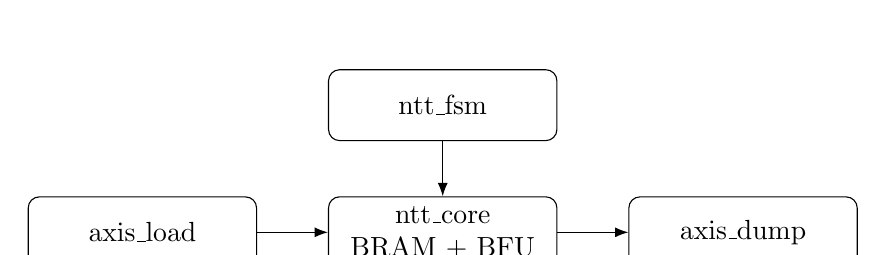
\begin{tikzpicture}[node distance=7mm and 9mm,>=Latex,
  box/.style={draw,rounded corners,minimum width=29mm,minimum height=9mm,align=center}]
\node[box] (load) {axis\_load};
\node[box,right=of load] (core) {ntt\_core\\BRAM + BFU};
\node[box,above=of core] (fsm) {ntt\_fsm};
\node[box,right=of core] (dump) {axis\_dump};
\draw[->] (load)--(core);
\draw[->] (fsm)--(core);
\draw[->] (core)--(dump);
\end{tikzpicture}
\end{center}

최종판은 transport-independent engine을 경계로 둔다.

\begin{center}
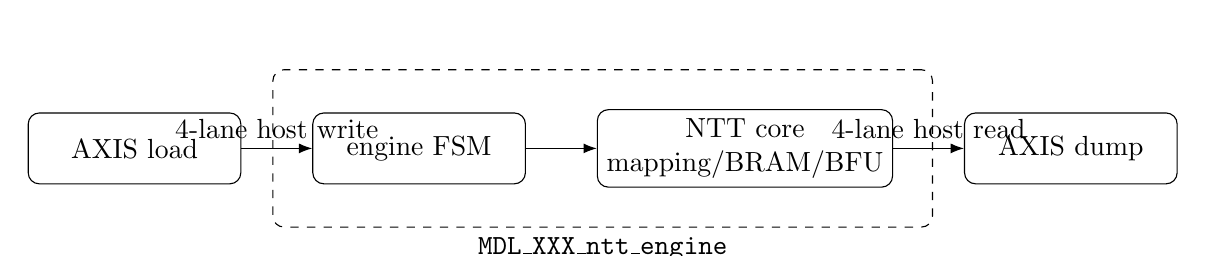
\begin{tikzpicture}[node distance=7mm and 9mm,>=Latex,
  box/.style={draw,rounded corners,minimum width=27mm,minimum height=9mm,align=center},
  group/.style={draw,dashed,rounded corners,inner sep=5mm}]
\node[box] (load) {AXIS load};
\node[box,right=of load] (fsm) {engine FSM};
\node[box,right=of fsm] (core) {NTT core\\mapping/BRAM/BFU};
\node[box,right=of core] (dump) {AXIS dump};
\node[group,fit=(fsm)(core),label=below:{\rtlfile{MDL\_XXX\_ntt\_engine}}] (eng) {};
\draw[->] (load)--node[above]{4-lane host write}(fsm);
\draw[->] (fsm)--(core);
\draw[->] (core)--node[above]{4-lane host read}(dump);
\end{tikzpicture}
\end{center}

AXI4-Stream top과 AXI BRAM Controller frontend가 같은 engine을 사용하므로,
interface 실험이 arithmetic schedule을 조용히 바꾸지 않는다. 이 분리는 직접적인
LUT 감소 기법이라기보다 비교의 신뢰성과 재사용성을 높이는 architecture 결정이다.

\section{최종 core의 한 transaction 흐름}

\begin{enumerate}
  \item \rtlfile{ntt\_addrgen}이 logical coefficient address와 zeta address를 만든다.
  \item \rtlfile{layout\_mapper}가 logical address를 physical side와 compact row로 바꾼다.
  \item 네 개의 true-dual-port coefficient BRAM에서 피연산자를 읽는다.
  \item 두 zeta를 packed ROM에서 동기식으로 읽는다.
  \item \rtlfile{unifiedBUT}이 선택된 radix/mode의 연산을 수행한다.
  \item valid/last와 physical tag가 13-stage result에 맞춰 이동한다.
  \item 반대 ping-pong set의 BRAM에 결과를 쓴다.
\end{enumerate}

이 흐름의 중요한 계약은 연산 중 mode가 고정되고, 새로운 transaction을 매 cycle
받을 수 있다는 점이다. latency는 길어질 수 있지만 \ii=1을 유지하면 layer의
steady-state 처리율은 유지된다.

\section{세 번의 설계 시점}

\begin{longtable}{L{31mm}L{44mm}L{86mm}}
\toprule
시점 & 관찰 & 다음 판단 \\
\midrule
\endhead
100~MHz baseline & timing 충족, memory address/control route가 최악 경로 & memory pin 앞 조합 경로를 register로 분할 \\
200~MHz 목표판 & DUMP 병목 제거 후 LOAD가 8-LUT/fanout-95 병목으로 이동, \wns $-3.563$~ns & 한 경로의 patch가 아니라 host memory command 전체를 재구성 \\
MC V5 150~MHz & compact memory, physical tag, shared host command, packed zeta, 재구성된 multiplier & 세 interface/standalone 범위에서 timing과 area 검증 \\
\bottomrule
\end{longtable}

이 과정은 timing closure가 ``한 번 pipeline을 넣고 끝내는 일''이 아님을 보여
준다. 한 병목을 제거하면 다음 실제 병목이 보인다. 매 iteration에서 새 report를
읽고, 원인 범위를 더 넓히거나 좁혀야 한다.

\section{최적화 동안 보존한 불변조건}

\begin{itemize}
  \item 두 \rtlfile{unifiedMUL}은 총 네 DSP48E1을 사용한다.
  \item mode가 고정된 동안 multiplier와 butterfly는 매 cycle 새 입력을 받는다.
  \item ping-pong layer는 읽는 set과 쓰는 set을 분리한다.
  \item logical coefficient 순서와 NTT/INTT 수학 결과는 유지한다.
  \item AXI backpressure 중 전송된 beat를 잃거나 중복하지 않는다.
\end{itemize}

최적화 전에 이 불변조건을 먼저 적어 두면 ``합성은 좋아졌지만 protocol 또는
cycle alignment가 바뀐'' 회귀를 빠르게 찾을 수 있다.

\chapter{Memory 경계의 Timing Closure}

\section{사례 1: DUMP address에서 BRAM까지}

100~MHz standalone baseline의 최악 setup path는 다음 경계였다.

\begin{lstlisting}[numbers=none]
u_dump/oDBG_RD1_ADDR_reg[2]
  -> u_core/u_bram3/.../ADDRARDADDR[6]
\end{lstlisting}

\begin{longtable}{L{38mm}rL{76mm}}
\toprule
항목 & 값 & 해석 \\
\midrule
Requirement & 10.000 ns & 100~MHz clock \\
Data path delay & 9.077 ns & setup 여유가 매우 작음 \\
Logic delay & 1.681 ns & 전체의 18.5\% \\
Route delay & 7.396 ns & 전체의 81.5\% \\
Logic levels & 8 & LUT2/3/4/5와 LUT6 네 개 \\
Post-route WNS & +0.273 ns & 100~MHz는 충족 \\
\bottomrule
\end{longtable}

주소는 layout side와 bank를 계산하고, LOAD/DUMP/CORE가 공유하는 BRAM port mux를
통과했다. logical address, bank selection, phase selection이 RAM address pin 앞
한 cycle에 모인 구조다. 200~MHz의 5~ns budget에는 맞지 않는다.

\subsection{첫 대응: address와 selection tag를 같이 등록한다}

중간 200~MHz 목표판은 DUMP address를 두 번 등록하고, bank/port tag도 BRAM
응답 cycle에 맞춰 등록했다. 핵심은 데이터만 늦추는 것이 아니라 \textbf{그
데이터를 선택할 metadata도 같이 늦추는 것}이다.

\begin{lstlisting}
dbg_addr_q  <= iDBG_RD_ADDR;
dbg_addr_q2 <= dbg_addr_q;
dbg_bank_q  <= dbg_bank;
dbg_bank_q2 <= dbg_bank_q;

case (dbg_bank_q)
  2'd0: begin bram0_ena = 1'b1; bram0_addra = dbg_addr_q2; end
  2'd1: begin bram1_ena = 1'b1; bram1_addra = dbg_addr_q2; end
  // ...
endcase
\end{lstlisting}

BRAM은 주소를 받은 다음 cycle에 동기식 read data를 내므로, output mux의 bank
tag는 address command보다 한 단계 뒤에 있어야 한다. 이 변경 때문에 AXI dump
valid pipeline도 3-stage에서 4-stage로 늘려 response data와 valid/TLAST를 다시
맞췄다.

\begin{warningbox}[pipeline 삽입의 실제 비용]
주소 register 하나를 넣는 변경은 주소만의 변경이 아니다. bank, port, valid,
last, FIFO reservation과 phase done 시점까지 같은 transaction을 가리키는지
확인해야 한다. 기능 simulation이 필요한 이유가 바로 이 cycle contract다.
\end{warningbox}

\section{사례 2: DUMP를 고치자 LOAD가 병목이 되었다}

DUMP 경로를 약 1~ns 수준으로 줄인 뒤, 200~MHz 목표판의 최악 경로는 LOAD
address에서 BRAM write-address pin으로 이동했다.

\begin{longtable}{L{41mm}rL{73mm}}
\toprule
항목 & 값 & 해석 \\
\midrule
Data path delay & 7.913 ns & 5~ns budget 초과 \\
Logic delay & 1.448 ns & 18\% 수준 \\
Route delay & 6.465 ns & 81\%, placement/routing 지배 \\
Logic levels & 8 LUT & bank/port/phase address mux \\
문제 net fanout & 95 & 넓은 memory control 분배 \\
Post-route WNS & $-3.563$ ns & 200~MHz 미충족 \\
\bottomrule
\end{longtable}

이 결과에서 얻을 교훈은 ``register를 더 넣자''보다 구체적이다. LOAD와 DUMP가
각자 mapper, bank rail, port rail을 만들고 마지막에 phase mux로 합쳐지면 RAM
주변에 넓은 조합 cone과 high-fanout net이 생긴다. 따라서 최종판은 host
transaction을 physical command로 먼저 바꾼 후 하나의 register bank에 저장했다.

\section{최종 구조: 공유되는 registered host command}

최종 \rtlfile{MDL\_XXX\_ntt\_core.v}의 핵심 register는 다음과 같다.

\begin{lstlisting}
reg        host_write_q;
reg [3:0]  host_valid_q;
reg [3:0]  host_side_q;
reg        host_set_q;
reg [LOCAL_ADDR_W-1:0] host_row0_q, host_row1_q,
                       host_row2_q, host_row3_q;
reg [D-1:0] host_data0_q, host_data1_q,
            host_data2_q, host_data3_q;
\end{lstlisting}

LOAD와 DUMP는 동시에 발생하지 않는 phase다. mapper 출력인 side와 compact row를
이 register에 저장하고, BRAM port mux는 등록된 physical command만 본다. 이
경계는 세 가지를 동시에 해결한다.

\begin{enumerate}
  \item logical-to-physical mapping을 BRAM pin 앞 경로에서 분리한다.
  \item LOAD/DUMP가 각각 소유하던 physical command rail을 공유한다.
  \item phase control의 큰 fanout을 register boundary에서 제한한다.
\end{enumerate}

4개씩 정렬된 host transaction에서 port pattern은 지원 mapping 모두 A,A,B,B로
고정된다. 따라서 세 lane의 port 선택은 state register가 아니라 상수 wire가 된다.

\begin{lstlisting}
wire host_port1_q = 1'b0;
wire host_port2_q = 1'b1;
wire host_port3_q = 1'b1;
\end{lstlisting}

동작 범위에서 항상 참인 불변조건을 찾아 runtime control을 없앤 사례다. 이
불변조건은 layout-mapper regression으로 모든 address에 대해 확인한다.

\section{control reduction tree를 memory path에서 제거한다}

최초 core는 pipeline이 비었는지 다음처럼 계산했다.

\begin{lstlisting}
wire pipe_nonempty = |valid_pipe;
assign oBUSY = iSTART | ag_running | req_valid_q |
               rd_valid_q | cap_valid_q | pipe_nonempty;
wire load_req = iLOAD_WE && !oBUSY;
\end{lstlisting}

긴 valid vector의 reduction OR가 \rtlfile{oBUSY}와 LOAD guard를 거쳐 BRAM address
mux까지 영향을 주었다. 중간판과 최종판은 입출 수를 세는 작은 occupancy
counter를 사용한다.

\begin{lstlisting}
reg [3:0] pipe_cnt;
wire pipe_nonempty = (pipe_cnt != 4'd0) | rd_valid_q;

if (but_enable) begin
  case ({rd_valid_q, wb_valid_int})
    2'b10: pipe_cnt <= pipe_cnt + 4'd1;
    2'b01: pipe_cnt <= pipe_cnt - 4'd1;
  endcase
end
\end{lstlisting}

counter는 FF와 작은 adder를 추가한다. 대신 wide reduction tree가 매 cycle의
memory control을 구동하지 않게 한다. timing을 위해 약간의 local state를 쓰는
trade-off다.

최종 LOAD path에서는 \rtlfile{!oBUSY} 조건도 제거했다. top-level phase FSM이
LOAD와 CORE를 상호 배타적으로 보장하므로 core 내부에서 같은 조건을 다시
계산할 필요가 없다. 이 제거는 안전성 전제를 hierarchy 계약으로 올린 것이다.
따라서 top-level FSM과 host write assertion을 함께 검증해야 한다.

\section{writeback mapping을 한 cycle 앞당긴 physical tag}

최초판은 logical address를 pipeline 끝까지 운반한 뒤 writeback 시점에 layout과
bank를 다시 계산했다. 최종판은 read request에서 \{side,row\} tag를 만들고
result와 같은 길이로 이동시킨다.

\begin{lstlisting}
req_tag_a_q <= {rd_side_a, rd_row_a};
// ... synchronous BRAM read and butterfly pipeline ...
wb_side_a_pre = a_pipe[PIPE_STAGES-2][ADDR_W-1];
wb_row_a_pre  = a_pipe[PIPE_STAGES-2][LOCAL_ADDR_W-1:0];
\end{lstlisting}

ping-pong set bit만 반전하면 최종 physical bank가 결정되므로 writeback pin 앞에
parity/affine mapping logic을 다시 둘 필요가 없다. ``계산 결과''뿐 아니라
``어디에 쓸 결과인가''도 pipeline data로 취급한 설계다.

\section{병목이 이동했는지 확인한다}

최종 150~MHz 결과에서 최악 경로는 더 이상 DUMP/LOAD address에서 BRAM pin으로
가는 경로가 아니다.

\begin{longtable}{L{42mm}L{49mm}rL{47mm}}
\toprule
범위 & 최악 경로 종류 & Data delay & WNS \\
\midrule
Standalone \rtlfile{MDL} & butterfly mode에서 modular add register & 6.522 ns & +0.089 ns \\
Complete AXI4-Stream & address-generator state에서 request tag & 6.366 ns & +0.075 ns \\
Complete BRAM controller & butterfly input에서 constant-multiply register & 6.550 ns & +0.006 ns \\
\bottomrule
\end{longtable}

이 표는 모든 경로가 넉넉하다는 뜻이 아니다. BRAM complete system은 6.666~ns
constraint에 0.006~ns만 남는다. 다만 처음의 memory-address 구조가 제거되어
다음 optimization 대상이 scheduler와 arithmetic 내부로 이동했음을 보여 준다.

\begin{checklistbox}
\begin{itemize}
  \item pipeline을 넣기 전 source/destination과 route 비율을 기록한다.
  \item address와 data를 선택하는 tag/valid/last를 같은 transaction으로 이동한다.
  \item 수정 후 이전 경로가 아니라 새 top-$N$ 경로를 다시 읽는다.
  \item high-fanout constraint를 넣기 전에 구조적으로 load 수를 줄일 수 있는지 본다.
  \item positive WNS뿐 아니라 zero failing endpoint와 hold도 확인한다.
\end{itemize}
\end{checklistbox}

\chapter{150 MHz에 연산을 담기까지}

\section{성공한 회로만 보면 설계 이유가 사라진다}

최종 RTL만 읽으면 register가 왜 그 위치에 있는지 알기 어렵다. 이 설계에서는
clock constraint를 바꾸고 top timing path를 다시 읽을 때마다 병목의 종류가
달라졌다. 남아 있는 report와 RTL milestone을 시간 순서로 놓으면 다음과 같다.

\begin{longtable}{L{22mm}L{50mm}L{68mm}}
\toprule
시점 & 관찰한 경로와 결과 & 다음 판단 \\
\midrule
최초 100~MHz &
DUMP address $\rightarrow$ BRAM address,
9.077 ns &
주소, bank, phase 선택을 BRAM pin 앞에서 끝내는 구조는 더 높은 주파수에
맞지 않았다. \\
초기 150~MHz &
mode select $\rightarrow$ radix-3 subtraction register,
$\wns=-0.338$ ns &
한 cycle에 연결된 23-bit carry 연산과 뒤쪽 선택을 분리해야 했다. \\
200~MHz 산술 실험 &
DSP product $\rightarrow$ ML-DSA intermediate register,
8.168 ns &
product 결합과 reduction digit 계산을 한 register 경계 안에 두지 않기로 했다. \\
최종 150~MHz &
standalone, AXI4-Stream, BRAM complete system 모두 timing 충족 &
목표 주파수를 검증된 production point로 고정하고 세 범위를 따로 보존했다. \\
\bottomrule
\end{longtable}

이 표의 각 행은 동일한 단일 변수 실험이 아니다. 개발 중 서로 다른 snapshot을
나열한 설계 일지다. 따라서 수치 차이 전체를 특정 RTL 변경의 효과로 해석하지
않는다. 여기서 사용할 수 있는 증거는 “그 시점의 top path가 무엇이었는가”와
“그 path의 조합 구조를 다음 RTL에서 어떻게 끊었는가”다.

\section{몇 ns가 걸리는지에 대한 직관}

RTL 연산 이름만으로 지연을 고정값처럼 외우면 안 된다. 같은 23-bit addition도
앞의 operand MUX, 뒤의 result MUX, fanout과 배치 위치에 따라 route delay가
달라진다. 이 프로젝트에서 실제 관찰한 path를 구성별로 나누면 다음과 같다.

\begin{longtable}{L{45mm}r r r L{45mm}}
\toprule
실제 경로 & Logic & Route & Total & 관찰한 구조 \\
\midrule
최초 DUMP address $\rightarrow$ BRAM &
1.681 ns & 7.396 ns & 9.077 ns &
8 LUT, route 81.5\% \\
초기 radix-3 subtraction result &
2.896 ns & 3.781 ns & 6.677 ns &
11 CARRY4를 포함한 13 levels \\
200~MHz ML-DSA intermediate &
4.600 ns & 3.568 ns & 8.168 ns &
12 CARRY4를 포함한 17 levels \\
최종 standalone modular-add register &
2.494 ns & 4.028 ns & 6.522 ns &
4 CARRY4를 포함한 7 levels \\
최종 BRAM system $1006x$ table-sum &
2.920 ns & 3.630 ns & 6.550 ns &
6 CARRY4를 포함한 10 levels \\
\bottomrule
\end{longtable}

여기서 얻는 실무적 직관은 세 가지다.

\begin{enumerate}
  \item 23-bit carry 연산 두 개와 mode selection이 이어진 path는 이
        implementation에서 6.677~ns였고 150~MHz에 들어가지 않았다.
  \item 더 복잡한 product 결합과 field 계산은 8.168~ns였다. 5~ns에
        맞추려면 식 정리만으로 부족하고 register 또는 DSP 내부 stage가 필요했다.
  \item logic이 짧아도 BRAM 주변처럼 route가 80\%를 넘으면 9~ns가 될 수 있다.
        반대로 “adder는 몇 ns”라는 표만으로 system timing을 예측할 수 없다.
\end{enumerate}

이 수치는 xc7z020 계열, Vivado 2020.2, 해당 placement와 constraint에서 얻은
경로 측정값이다. 다른 device, speed grade, floorplan과 fanout에는 그대로
대입하지 않는다. 설계 초기에 필요한 것은 절대값 암기가 아니라
“carry가 몇 번 직렬인가”, “MUX가 carry 앞뒤 어디에 있는가”,
“logic보다 route가 큰가”를 구분하는 감각이다.

\section{실패 1: subtract와 correction을 한 cycle에 연결했다}

modular subtraction은 식으로 쓰면 짧다.
\[
d=a-b,\qquad r=
\begin{cases}
d+q,&d<0,\\
d,&d\ge0.
\end{cases}
\]
그러나 23-bit RTL에서 raw subtraction, borrow 선택, conditional addition과
mode-dependent result 선택이 같은 register 앞에 놓이면 carry chain 두 개와
MUX가 직렬로 합성될 수 있다.

초기 150~MHz post-route report의 top path는 mode register에서
radix-3 subtraction result register까지였다. 6.667~ns requirement에서 data
path가 6.677~ns였고, logic 2.896~ns와 route 3.781~ns를 사용했다. 13 logic
levels 가운데 CARRY4가 11개였다. setup slack은 $-0.338$~ns였다. 이 결과는
“subtractor 하나가 느리다”보다 다음 사실을 보여 준다.

\begin{itemize}
  \item carry 결과를 고르는 mode MUX도 같은 path의 일부다.
  \item 산술 depth와 route가 모두 커서 placement directive만으로 해결하기 어렵다.
  \item source가 mode register라는 사실은 연산뿐 아니라 control fanout도
        함께 줄여야 함을 뜻한다.
\end{itemize}

최종 RTL은 모든 modular subtraction에 새 stage를 추가하지 않았다. multiplier
앞에서 일찍 필요한 두 general difference만 C1과 C2로 나눴다.

\begin{lstlisting}
// C1: raw subtraction and borrow
raw0_c1    <= {1'b0, b} - {1'b0, a};
borrow0_c1 <= raw0[D];

// C2: conditional correction
corrected = {1'b0, raw0_c1[D-1:0]} + {1'b0, q};
d0_c2     <= borrow0_c1 ? corrected[D-1:0]
                        : raw0_c1[D-1:0];
\end{lstlisting}

C2는 이 rail에서 원래 alignment에 쓰이던 자리였다. 그러므로 새 latency를
더하지 않고 기존 register의 일을 바꾸어 두 carry chain을 서로 다른 cycle에
배치했다. 이 사례에서 핵심 판단은 “pipeline을 한 단계 늘린다”가 아니라
\textbf{이미 존재하는 alignment stage에 실제 연산을 배치한다}는 것이다.

또한 arithmetic result인 radix-3의 $E$와 $S$를 첫 register에서 공통 A/C rail에
바로 합치지 않았다. carry chain 직후에 mode MUX가 붙기 때문이다. 첫 register는
분리하고, 다음 경계에서 이미 등록된 값끼리 merge했다.

\section{실패 2: ML-DSA product 결합과 digit 계산을 함께 수행했다}

200~MHz 실험의 한 post-route top path는 DSP48E1의 product output에서
\rtlfile{a\_tmp\_buf} register까지였다. 5.000~ns requirement에 data path는
8.168~ns, logic levels는 17개였고 그중 CARRY4가 12개였다. slack은
$-3.171$~ns였다.

당시 조합 cone은 low product의 정렬된 high part와 다른 partial product를
더한 뒤, 그 결과에서 여러 field sum을 연속으로 만들었다. RTL의 수식은 맞고
simulation도 통과했지만, Vivado가 본 물리 경로에는 긴 carry chain이 남았다.
“중간 wire 이름을 여러 개 둔다”는 것은 pipeline이 아니다. register edge가
없으면 모든 식은 여전히 한 cycle의 경로다.

최종 six-stage \rtlfile{unifiedMUL}은 일을 다음처럼 나눈다.

\begin{enumerate}
  \item DSP0가 16-bit low product를 계산한다.
  \item DSP1의 MREG/PREG가 ML-DSA high partial product와 aligned cross-sum을
        받아 외부 fabric의 긴 product-adder 경계를 줄인다.
  \item C3에서 $H_0+H_1$을 한 번 계산하고 다음 high-part 식에서도 재사용한다.
        별도 24-bit addition 대신 두 번째 carry chain을 14 bit로 제한한다.
  \item C4에서 segmented residual, C5에서 base/correction addition,
        C6에서 constant-selected canonical correction을 수행한다.
\end{enumerate}

마지막 correction도 high digit과 low digit을 각각 고치는 branch로 표현했을 때
합성기가 branch MUX와 carry를 깊게 합쳤다. 최종판은 범위 판정으로
$0,+q,-q,-2q$ 중 correction constant 하나를 고르고 signed addition 한 번만
수행한다. 수학적으로 같은 식 가운데 FPGA에서 carry와 MUX가 직렬로 놓이지
않는 표현을 선택한 것이다.

\section{실패 3: Montgomery의 다섯 operand를 한 번에 더했다}

초기 R16 Montgomery path는 선택된 네 shifted operand를 더해
$c_qT\bmod 2^9$를 만들고, 같은 조합 경로에서 $T[15:7]$까지 더해
$u[15:7]$을 완성했다.

\begin{lstlisting}
shift_sum = op0 + op1 + op2 + op3;
u_hi      = shift_sum + T[15:7];
\end{lstlisting}

operand 폭은 9 bit로 작지만 다섯 항의 mode selection과 addition이 한 cycle에
모였다. 최종판은 C2에 $c_qT\bmod512$만 등록하고, 등록된 $T[15:7]$은 다음
DSP-input cycle에서 더한다.

\begin{lstlisting}
// C2 register
corr9_c2 <= op0 + op1 + op2 + op3;
t_c2     <= T;

// following DSP-input cycle
u_hi = t_c2[15:7] + corr9_c2;
u    = {u_hi, t_c2[6:0]};
\end{lstlisting}

DSP1이 ML-DSA와 Montgomery mode에서 서로 다른 cycle 역할을 갖는다는 schedule을
이용했으므로 six-cycle latency와 \ii=1을 유지했다. pipeline 최적화는 연산을
기계적으로 반으로 자르는 일이 아니라, 다음 hard block이 operand를 받는
시점까지 포함해 cut 위치를 정하는 일이다.

\section{실패 4: 상수곱에 stage 하나를 더 넣자 기능이 깨졌다}

NTRU+의 고정 상수곱은 처음에 shifted partial product 일곱 개와
$q=4096-639$를 이용한 여러 fold를 두 cycle에 배치했다. adder tree를
balanced form으로 다시 써도 product와 modular fold의 carry depth 자체는
남았다. 이후 작은 input field를 table로 바꾸어 carry chain을 table output의
합과 한 번의 correction으로 줄였다. 최종 $1006x\bmod3457$ 회로는
6-bit field 두 개의 table과 12-bit modular addition을 사용한다.

더 높은 주파수 실험에서는 이 상수곱을 세 stage로 늘려 보았다. 개별 block의
조합 depth는 줄지만 radix-3/삼항식 branch는 상수곱 결과와 별도의 difference
rail이 같은 cycle에 도착한다고 가정했다. 상수곱만 한 cycle 늦어지자 NTRU+
INTT 결과가 어긋났다.

선택지는 두 가지였다.

\begin{enumerate}
  \item 관련된 모든 branch와 metadata를 한 cycle 더 지연한다.
  \item 두-cycle 계약을 유지하고 연산 표현을 바꾼다.
\end{enumerate}

첫 선택은 공통 alignment FF와 전체 latency를 늘린다. 최종판은 두 번째를
택했다. raw subtraction의 underflow correction을 table 앞 12-bit adder로
수행하지 않고, underflow일 때 더해야 하는 상수 효과
$-1006\times639\equiv168\pmod{3457}$를 table 선택에 미리 반영했다.
그 결과 correction carry chain 하나를 table data selection으로 바꾸면서
두-cycle arrival contract를 보존했다.

이 실패는 “register를 넣으면 timing은 좋아진다”는 문장이 불완전함을
보여 준다. multi-branch pipeline에서는 값, valid, mode, destination tag와
parallel operand가 같은 transaction으로 다시 만나는 cycle까지 함께 바뀐다.

\section{실패 5: 연산기를 최대한 공유했더니 더 커졌다}

한 실험판은 네 개의 runtime-generic folded ALU에 23-bit와 12-bit 연산을 모두
모으고, raw/correction two-pass register와 공통 delay rail을 두었다. 연산기
개수만 세면 매력적이지만 실제 FPGA 비용은 다음 위치로 이동했다.

\begin{itemize}
  \item generic ALU 앞의 wide operand crossbar
  \item carry chain 뒤의 mode-dependent result MUX
  \item 여러 stage와 mode로 퍼지는 select fanout
  \item latency가 다른 branch를 끝까지 끌고 가는 alignment FF
\end{itemize}

NTRU+ lazy reduction도 다섯 internal correction을 제거하는 대신 intermediate가
13--14 bit로 넓어졌다. multiplier와 constant-multiplier 입력이 커지고 output
canonicalization이 다시 필요했다. 최종 output에서 제거했던 adder/MUX가
돌아오므로 해당 branch의 순 area 이득이 사실상 사라졌다.

최종 구조는 큰 자원과 시점이 정확히 맞는 연산을 공유한다. 두 DSP, DSP
register, final correction addition은 공유한다. NTRU+의 cycle-local add/sub는
12 bit로 남긴다. 이 경험에서 나온 기준은 다음과 같다.

\begin{tradeoffbox}[공유 여부를 결정하는 기준]
연산기 개수만 비교하지 않는다. 공유 전후의 operand MUX 폭, result MUX 위치,
mode fanout, alignment register와 placement 거리까지 합쳐서 비교한다.
\end{tradeoffbox}

\section{implementation directive만으로 150 MHz가 되지 않았다}

중간 RTL을 Zynq-7020에 standalone OOC로 구현했을 때 default flow의
150~MHz WNS는 $-0.374$~ns였다. synthesis retiming과 timing-oriented
place/route directive를 적용하면 $-0.152$~ns까지 회복했지만 여전히
timing은 닫히지 않았다. 같은 flow에서 140~MHz는 $+0.026$~ns였다.

이 수치는 directive가 쓸모없다는 뜻이 아니다. RTL의 register, MUX, fanout
구조를 고친 뒤 implementation flow가 나머지 placement/routing margin을
회복한다. 최종 150~MHz 결과는 두 작업을 함께 적용한 결과다.

300~MHz 실험에서는 3.333~ns constraint에서 synthesis WNS $-7.170$~ns와
RAMB36E1 pulse-width slack $-0.551$~ns가 관찰되었다. 이 implementation
point는 route를 진행하지 않았다. pulse-width violation은 조합 path에 register를
더 넣는 것으로 해결되지 않기 때문이다. 목표 주파수를 올리는 실험도
\textbf{RTL로 고칠 path}, \textbf{clock/device primitive 제한},
\textbf{기능 정렬 비용}을 구분해 중단 기준을 세워야 한다.

\begin{checklistbox}
\begin{itemize}
  \item 실패한 run도 requirement, WNS, source, destination, logic levels,
        logic/route 비율을 남긴다.
  \item 한 cycle 식에서 carry chain이 몇 번 이어지는지 회로로 다시 그린다.
  \item 빈 alignment stage를 먼저 찾고 새 stage 추가는 그다음에 검토한다.
  \item 한 branch의 latency를 바꾸면 parallel data와 metadata의 합류 cycle을
        testbench에서 확인한다.
  \item 공유 실험은 ALU 수뿐 아니라 MUX, fanout, FF와 route까지 비교한다.
  \item directive로 얻은 margin과 RTL 구조 변경의 효과를 같은 것으로 쓰지 않는다.
\end{itemize}
\end{checklistbox}

\chapter{Memory와 Metadata의 Area 최적화}

\section{사례 1: BRAM inference가 먼저다}

초기 synthesis는 true-dual-port memory의 두 write port를 합성기가 인식하는
형태로 표현하지 못해 RAM을 register로 풀었다. 네 bank hierarchy가 각각 약
27--29k LUT와 47,150 FF를 사용했고, 전체는 device 용량을 훨씬 초과했다.
이때의 우선순위는 address 폭 축소나 mux 미세 최적화가 아니라 inference
template 수정이다.

최종 \rtlfile{MDL\_XXX\_bram\_dp.v}는 port별 synchronous process를 분리한다.

\begin{lstlisting}
(* ram_style = "block" *) reg [DATA_W-1:0] mem [0:DEPTH-1];

always @(posedge iSYS_CLK) begin : PORT_A
  if (iENA) begin
    if (iWEA) mem[iADDRA] <= iDINA;
    oDOUTA <= mem[iADDRA];
  end
end

always @(posedge iSYS_CLK) begin : PORT_B
  if (iENB) begin
    if (iWEB) mem[iADDRB] <= iDINB;
    oDOUTB <= mem[iADDRB];
  end
end
\end{lstlisting}

\rtlfile{ram\_style} attribute만 붙이는 것으로 부족하다. port semantics가
primitive가 지원하는 동작과 맞아야 한다. read-first 동작과 same-row dual write가
없다는 scheduler 계약도 simulation assertion으로 남긴다.

\section{사례 2: logical depth와 physical depth를 분리한다}

최초 coefficient bank parameter는 11-bit address, depth 2048이었다. 최대 transform
길이는 1152이지만 네 physical bank가 각각 logical address 전체를 받을 수 있게
작성되어 있었다. 2048$\times$23 true-dual-port bank 하나는 7-series에서
RAMB36과 RAMB18의 조합으로 구현되었고, 네 bank가 6 BRAM-tile equivalents를
소비했다.

최종 mapping은 logical address $x$를 side와 row로 나눈다.
\[
row=x[10:1],\qquad side=x_0\oplus x_k.
\]
지원 transform에서 최대 row는 575이므로 각 bank는 576$\times$23이면 충분하다.
이 크기는 RAMB36E1 하나에 들어가며 네 coefficient bank는 총 4 RAMB36이 된다.

\subsection{왜 정보가 사라지지 않는가}

$row$에는 $x_k$가 남아 있다($k\ge1$). 그러므로
\[
x_0=side\oplus x_k
\]
로 제거한 bit 0을 복원할 수 있다. 즉 $(side,row)$는 logical address와 일대일
대응한다. 단순히 address LSB를 버린 것이 아니라, 그 정보를 side에 보존한
compact mapping이다.

\begin{lstlisting}
assign oSIDE       = addr[0] ^ addr[k];
assign oLOCAL_ADDR = addr[ADDR_W-1:1];
\end{lstlisting}

실제 RTL은 variable $k$ 대신 4, 6, 7의 고정 tap을 case로 선택한다. mapping별
bijection, row bound, radix-2 bank balance를 exhaustive test로 확인한다.

\section{사례 3: scheme별 ROM을 word packing으로 통합한다}

최초 \rtlfile{zeta\_rom}은 ML-KEM, ML-DSA, HAETAE, NTRU+768,
NTRU+864/1152 ROM을 모두 instantiate한 뒤 mode mux로 출력을 선택했다. 합성
결과의 twiddle storage는 RAMB18 세 개, 즉 1.5 tile이었다.

최종판은 2048$\times$32의 packed image 하나를 두 synchronous read port로
읽는다. 저장 구간은 다음과 같다.

\begin{longtable}{L{37mm}r r L{78mm}}
\toprule
Mode & Base word & Words & Packing \\
\midrule
ML-DSA & 0 & 256 & 23-bit value 1개/word \\
HAETAE & 256 & 128 & 16-bit value 2개/word \\
ML-KEM & 384 & 64 & 12-bit value 2개/word \\
NTRU+768 & 448 & 96 & 12-bit value 2개/word \\
NTRU+864/1152 & 544 & 144 & 12-bit value 2개/word \\
Falcon forward & 688 & 512 & 16-bit value 2개/word \\
Falcon inverse & 1200 & 512 & 16-bit value 2개/word \\
\bottomrule
\end{longtable}

총 1712 word이므로 2048-word memory에 들어간다. narrow mode의 logical address
LSB가 word 안의 low/high slot을 고른다.

\begin{lstlisting}
phys_w = base_w + logical_addr[10:1];
slot_w = logical_addr[0];

out = slot_q ? word_q[31:16] : word_q[15:0];
\end{lstlisting}

packed ROM은 두 RAMB36을 사용한다. twiddle memory만 보면 1.5 tile에서 2 tile로
0.5 tile 증가했지만, Falcon forward/inverse table까지 포함한다. coefficient
bank가 6 tile에서 4 tile로 줄어 전체 accelerator memory는 7.5 tile에서 6
tile로 1.5 tile 감소했다. 부분별 증감을 나눠 보아야 올바른 설명이 된다.

\section{사례 4: pipeline metadata도 area다}

data path만 세면 control storage를 놓치기 쉽다. 최초 core는 네 lane의
\rtlfile{va/vb/vc/vd}를 각각 12-stage pipeline으로 운반했고, BRAM read 뒤에
data/address/zeta를 다시 capture하는 register group도 있었다.

최종 transaction에서는 A/B/C lane이 항상 유효하고 radix-3일 때만 D가 없다.
따라서 tail valid는 layer-static butterfly mode로 계산한다.

\begin{lstlisting}
wire ctl_is_r3 = (ctl_but_sel_q == BUT_R3_NTT) ||
                 (ctl_but_sel_q == BUT_R3_INTT);
wire wb_lane_d_valid = !ctl_is_r3;
\end{lstlisting}

최종 13-stage 기준으로 네 lane-valid shift register 52 FF를 제거한다. 이 숫자는
해당 register의 구조적 감소량이며, 전체 FF delta와 동일시하지 않는다. 다른
pipeline과 interface register도 동시에 바뀌었기 때문이다.

read data와 synchronous zeta output은 butterfly C1 register로 직접 들어가도록
정렬하여 duplicate capture stage도 제거했다. pipeline register를 무조건 줄인
것이 아니라, 같은 cycle boundary가 두 번 존재하는 부분을 찾은 것이다.

\section{사례 5: 계측 logic을 production에서 생성하지 않는다}

LOAD/CORE/DUMP/TOTAL cycle counter는 개발 중 유용하지만 accelerator protocol의
필수 기능은 아니다. 최종 top은 parameterized generate로 네 32-bit counter와
incrementer를 production configuration에서 제거한다.

\begin{lstlisting}
generate
  if (ENABLE_PERF_COUNTERS != 0) begin : GEN_PERF_COUNTERS
    // four 32-bit cycle counters
  end else begin : GEN_NO_PERF_COUNTERS
    always @(posedge iSYS_CLK) begin
      oLOAD_CYCLES  <= 0;
      oCORE_CYCLES  <= 0;
      oDUMP_CYCLES  <= 0;
      oTOTAL_CYCLES <= 0;
    end
  end
endgenerate
\end{lstlisting}

하위 AXI load/dump beat counter도 같은 parameter를 사용한다. 검증용 관측성을
유지하면서 release hardware에 incrementer와 fanout을 남기지 않는 방법이다.

\section{Area 감소를 설명하는 올바른 문장}

최초 standalone과 최종 standalone의 역사적 결과는 LUT 5,278에서 4,736,
FF 3,072에서 2,792, BRAM tile 7.5에서 6.0, DSP 4에서 4다. 각각 10.3\%,
9.1\%, 20.0\% 감소와 DSP 동일이다. 그러나 package, top boundary, clock가
완전히 일치하는 단일 변수 실험은 아니다.

따라서 다음과 같이 쓴다.

\begin{goodbox}[권장 해석]
최종 implementation point는 최초 standalone archive보다 542 LUT, 280 FF,
1.5 BRAM tile을 적게 사용하고 같은 네 DSP를 사용한다. compact coefficient
mapping은 bank당 RAMB18을 제거했고, 다른 LUT/FF 변화에는 arithmetic,
scheduler, metadata, wrapper 차이가 함께 포함된다.
\end{goodbox}

특정 RTL 변경 하나가 전체 542 LUT를 줄였다고 쓰려면 그 변경만 다른 matched
run이 추가로 필요하다.

\chapter{Modular Arithmetic의 자원 공유와 Pipeline}

\section{설계 목표를 연산식과 자원으로 동시에 적는다}

최종 \rtlfile{unifiedMUL}의 목표는 두 종류의 modular multiplication을 같은
두 DSP48E1과 arithmetic/register path에서 실행하는 것이다.

\begin{itemize}
  \item ML-DSA: $q=8{,}380{,}417$, 23-bit operand path
  \item Narrow primes: R16 Montgomery multiplication, $R=2^{16}$
  \item Narrow modulus: ML-KEM 3,329, HAETAE 64,513, NTRU+ 3,457,
        Falcon 12,289
  \item Latency: six pipeline stages
  \item Throughput: mode가 유지되는 동안 매 cycle 새 입력 수락, \ii=1
\end{itemize}

하나의 \rtlfile{unifiedBUT}은 \rtlfile{unifiedMUL} 두 개를 사용하므로 전체
butterfly arithmetic은 DSP48E1 네 개를 사용한다.

\section{DSP0: 공통 low product}

두 path 모두 먼저 $A$와 $B$의 low 16-bit product를 필요로 한다.

\begin{lstlisting}
(* use_dsp = "yes" *) wire [38:0] c1_mul_lo_w;
assign c1_mul_lo_w = iA[22:0] * iB[15:0];

always @(posedge iSYS_CLK)
  if (iFSM_START) c1_mul_lo_r <= c1_mul_lo_w;
\end{lstlisting}

ML-DSA에서는 23-bit $B$를 low 16-bit와 high 7-bit로 분할한다.
\[
A B=A B_{lo}+2^{16}A B_{hi}.
\]
DSP0의 low product와 DSP1의 high partial product를 정렬해 더한다. Narrow-prime
mode에서는 DSP0 output의 low 32 bit가 $T=A B$다.

\section{Narrow-prime path: R16 Montgomery multiplication}

Narrow mode는 다음 연산을 수행한다.
\[
T=A B,\qquad
u=Tq^{-1}\bmod 2^{16},\qquad
t=\frac{T-uq}{2^{16}}.
\]
$t<0$이면 $q$를 한 번 더해 canonical result를 만든다. 네 modulus는 모두
$q\equiv1\pmod{2^7}$을 만족하므로
\[
q^{-1}=1+2^7c_q\pmod{2^{16}}
\]
로 쓸 수 있다. 따라서 $u$의 low 7 bit는 $T$의 low 7 bit와 같고, high 9 bit는
선택된 shift와 9-bit addition으로 계산할 수 있다.

실제 RTL은 mode별로 필요한 shifted value를 고른 뒤 하나의 9-bit 합에 넣는다.

\begin{lstlisting}
case (mode)
  CTL_KYBER: begin op0 = -m3; op1 = m5; op2 = m6; end
  CTL_HAETAE:begin op0 =  m4;                    end
  CTL_NTRU:  begin op0 =  m2; op1 = m3;
                    op2 =  m5; op3 = m7;          end
  CTL_FALCON:begin op0 = -m2; op1 = -m3;          end
endcase
corr9 = op0 + op1 + op2 + op3;
\end{lstlisting}

여기서 $m_2,\ldots,m_7$은 $T$의 일부 bit를 고정 shift한 9-bit 값이다. 9-bit
wraparound가 modulo 512 연산을 제공한다. 네 modulus마다 넓은 constant multiplier를
병렬로 만든 뒤 고르는 구조를 피하고, mode select와 작은 addition을 공유한다.

\section{DSP1: mode별 곱과 정렬 산술 공유}

두 번째 DSP는 mode에 따라 다른 역할을 한다.

\begin{longtable}{L{29mm}L{57mm}L{75mm}}
\toprule
Mode & DSP1 multiplication & DSP ALU/PREG 동작 \\
\midrule
ML-DSA & $A\times B_{hi}$ & DSP0 low product의 정렬된 high 부분과 덧셈 \\
Narrow prime & $u\times q$ & 정렬된 $T$에서 $u q$를 뺌 \\
\bottomrule
\end{longtable}

최종 synthesis branch는 DSP48E1의 MREG, ALU, PREG를 사용한다. ML-DSA와
Montgomery path의 fabric mux를 multiplier 바로 앞에 깊게 두지 않고 DSP의
A/D/C 입력과 ALUMODE/INMODE로 역할을 바꾼다. simulation branch는 같은 latency의
behavioral multiplication과 register를 사용하므로, 두 branch가 bit-accurate하고
cycle-accurate한지 regression에서 함께 확인해야 한다.

\section{공유 register는 live bit를 기준으로 설계한다}

각 stage의 payload 폭은 두 mode의 필요한 정보를 담을 만큼만 잡는다.

\begin{longtable}{C{15mm}L{52mm}L{94mm}}
\toprule
Stage & ML-DSA에서 보존할 값 & Narrow mode에서 보존할 값 \\
\midrule
C1 & 23$\times$16 low product & $T=A B$ \\
C2 & low product 일부 & $T$와 $c_qT\bmod512$ \\
C3 & quotient 준비용 high/low 조각 & DSP1 subtraction용 정렬된 $T$ \\
C4 & residual과 borrow 정보 & $T-uq$는 DSP1 PREG에 유지 \\
C5 & base-minus-borrow 결과 & negative result에 조건부 $+q$ \\
C6 & ML-DSA canonical correction & C5 narrow result 출력 \\
\bottomrule
\end{longtable}

두 mode가 같은 cycle에 동시에 실행되지 않으므로 payload의 live range가 겹치지
않는 bit는 공유할 수 있다. 다만 mode mux가 wide payload 전체에 생기지 않도록
양쪽에서 실제로 소비되는 low part만 선택하고, 한 mode에서 의미 없는 upper
part는 다른 mode 값을 그대로 연결한다.

\section{최종 correction addition 공유}

C5에서는 ML-DSA의 base-minus-borrow와 narrow Montgomery result의 조건부 $+q$를
하나의 signed 18-bit adder로 표현한다.

\begin{lstlisting}
shared_a = is_dili ? sign_extend(dili_base)
                   : sign_extend(mont_quotient);
shared_b = is_dili ? -borrow
                   : (mont_negative ? mont_q : 0);
shared_sum = shared_a + shared_b;
\end{lstlisting}

공유 가능성은 ``둘 다 덧셈처럼 보인다''에서 나오지 않는다. 두 연산이 같은
pipeline stage에 있고, mode가 transaction 동안 고정되고, 필요한 signed range가
18 bit 안에 들어간다는 세 조건에서 나온다.

\section{ML-DSA path의 폭을 줄이는 방법}

ML-DSA modulus는
\[
2^{23}\equiv 2^{13}-1\pmod q
\]
관계를 갖는다. 최종 RTL은 23-bit operand split으로 얻은 product 조각을 13-bit
radix 위치에 맞춰 재배열하고, 필요한 low subtraction과 high signed addition을
나눠 계산한다. 이는 알려진 modulus relation을 shared datapath에 맞게 배치한
것이며 새로운 reduction algorithm을 주장하는 근거가 아니다.

중요한 RTL 습관은 중간값의 증명된 범위를 사용해 폭을 정하고 assertion으로
남기는 것이다. 예를 들어 signed high base와 final canonical range가 예상 범위를
벗어나면 simulation에서 즉시 error를 발생시킨다. 이런 assertion은 합성에서
제거되므로 production area에는 포함되지 않는다.

\section{산술 timing의 현재 위치}

최종 standalone 150~MHz 최악 경로는 mode register에서 butterfly modular-add
register까지이며, 7 logic levels와 6.522~ns data delay를 보였다. complete BRAM
system 최악 경로도 butterfly input에서 constant-multiply register까지 10 logic
levels, 6.550~ns다. memory-address path가 정리된 뒤 arithmetic이 다시 timing
closure의 중심이 된 것이다.

다음 개선을 시도한다면 mode fanout, constant-add partition, stage boundary를
matched OOC run으로 비교해야 한다. 단순히 DSP를 더 쓰거나 pipeline latency를
늘리기 전에 \ii=1, 네-DSP limit, layer cycle 계약을 함께 보존해야 한다.

\begin{checklistbox}
\begin{itemize}
  \item mode별 수식을 먼저 쓰고 같은 cycle의 공통 연산을 찾는다.
  \item operand와 중간값의 signed range를 증명해 register 폭을 정한다.
  \item DSP 내부 MREG/PREG와 fabric register의 경계를 따로 센다.
  \item mode mux가 DSP/carry 앞 critical path에 붙는지 report로 확인한다.
  \item latency와 initiation interval을 별도 지표로 검증한다.
\end{itemize}
\end{checklistbox}

\chapter{Scheduler, memory mapping, interface}

\section{연산량보다 빈 cycle을 먼저 센다}

같은 butterfly 수라도 layer 시작, BRAM read, pipeline fill/drain, 다음 layer
descriptor 준비 때문에 cycle 수가 달라진다. 최종 radix-2 schedule의 관측식은
다음처럼 정리된다.
\[
C_{core}=L\,(N_{issue/layer}+15).
\]
ML-KEM은 7개 layer와 layer당 64 issue로 $7(64+15)=553$ cycle,
ML-DSA/HAETAE는 8개 layer로 $8(64+15)=632$ cycle이다. 이 식의 15는 단일
butterfly latency만 뜻하지 않는다. address issue부터 final writeback과 layer
전환까지의 관측 overhead다.

최종 FSM은 다음 layer descriptor를 미리 계산하고, 마지막 writeback edge의
lookahead로 다음 layer를 시작한다. address generator도 first transaction seed를
descriptor에 포함해 layer 시작 뒤의 별도 준비 cycle을 줄인다.

\section{NTRU+864의 half-empty issue 제거}

NTRU+864의 특수 step-3 구간을 일반 schedule로 표현하면 일부 transaction에서
lane을 충분히 사용하지 못한다. 최종 \rtlfile{ntt\_addrgen}은
\rtlfile{ADDR\_MODE\_N864\_STEP3}를 별도로 두어 유효 coefficient 조합을 직접
발행한다. 이는 memory layout 자체를 바꾸는 mode가 아니다. logical address
schedule만 바꾸고 affine mapping은 유지한다.

이 구분 덕분에 scheduler test는 issue address/valid를 검사하고, mapper test는
bijection/bank conflict를 독립적으로 검사할 수 있다. schedule과 physical layout을
한 always block에 섞으면 어느 쪽의 오류인지 분리하기 어렵다.

\section{Core-cycle 결과}

\begin{longtable}{L{31mm}r r r r}
\toprule
Configuration & 최초 cycle & 최종 cycle & Cycle 감소 & 100/150 MHz 시간 감소 \\
\midrule
ML-KEM-256 & 557 & 553 & 0.7\% & 33.8\% \\
ML-DSA-256 & 636 & 632 & 0.6\% & 33.8\% \\
HAETAE-256 & 636 & 632 & 0.6\% & 33.8\% \\
NTRU+768 & 1,709 & 1,513 & 11.5\% & 41.0\% \\
NTRU+864 & 2,053 & 1,761 & 14.2\% & 42.8\% \\
NTRU+1152 & 2,605 & 2,313 & 11.2\% & 40.8\% \\
\bottomrule
\end{longtable}

마지막 열은 최초 100~MHz와 최종 150~MHz implementation point를 사용한 core-only
시간이다. radix-2-only mode는 cycle 감소가 작고 주파수 상승 효과가 중심이다.
Mixed-radix NTRU+는 scheduler cycle 감소가 추가로 기여한다.

\section{AXI LOAD: beat 안의 병렬성을 memory lane으로 전달한다}

64-bit AXI input 한 beat는 ML-DSA에서 32-bit coefficient 두 개, narrow mode에서
16-bit coefficient 네 개를 담는다. 최종 loader는 accepted beat마다 최대 네
logical write를 같은 cycle에 만든다.

\begin{lstlisting}
oLOAD_WE  <= 1'b1;  oLOAD_ADDR  <= coeff_q;
oLOAD1_WE <= 1'b1;  oLOAD1_ADDR <= coeff_q + 1;
oLOAD2_WE <= !mldsa;oLOAD2_ADDR <= coeff_q + 2;
oLOAD3_WE <= !mldsa;oLOAD3_ADDR <= coeff_q + 3;
\end{lstlisting}

지원하는 모든 $N$이 packing factor로 정확히 나누어지므로 각 lane의 upper-bound
comparator를 반복할 필요가 없다. 한 번의 \rtlfile{all\_issued/final\_accept}
판정으로 충분하다. 불변조건을 이용해 세 개의 11-bit 비교기를 제거한 사례다.

\rtlfile{oWS\_TREADY}는 receive state에서 항상 1이고 내부 bubble을 삽입하지
않는다. 따라서 source가 TVALID를 연속으로 주면 매 cycle 한 beat를 받는다.

\section{AXI DUMP: backpressure보다 먼저 reservation한다}

BRAM request는 발행 후 취소할 수 없다. downstream \rtlfile{TREADY}가 내려간
뒤 FIFO가 꽉 차면 이미 날아오는 response를 버리게 된다. 최종 dump는 현재
FIFO count만 보지 않고, 아직 도착하지 않은 request까지 slot을 예약한다.

\begin{lstlisting}
wire pop       = (count_q != 0) && iWM_TREADY;
wire can_issue = (credit_q != 0) || pop;
wire issue     = active_q && !all_issued && can_issue;

case ({issue,pop})
  2'b10: credit_q <= credit_q - 1'b1;
  2'b01: credit_q <= credit_q + 1'b1;
endcase
\end{lstlisting}

같은 cycle에 pop이 있으면 그 slot을 새 request에 즉시 재사용한다. 정상
\rtlfile{TREADY=1} 상태에서 refill bubble 없이 \ii=1을 유지하면서, 임의의
backpressure에서는 overflow를 막는다. FIFO payload는 reset하지 않는다.
\rtlfile{count\_q=0}이 모든 오래된 entry를 invalid로 만들기 때문에 payload reset을
없애 LUTRAM inference와 packing을 돕는다.

\section{Interface 두 개를 비교하는 법}

AXI4-Stream과 AXI BRAM Controller는 같은 engine을 사용하지만 PS--PL data movement가
다르다. 따라서 비교에는 두 층이 있다.

\begin{itemize}
  \item \textbf{Core-only}: 같은 engine의 cycle와 standalone area
  \item \textbf{End-to-end}: configuration, cache handling, DMA/MMIO transfer,
        polling, output availability를 포함한 board 시간
\end{itemize}

최종 complete-system에서 stream 쪽은 AXI DMA MM2S/S2MM payload FIFO를 포함한다.
MM2S FIFO는 68 bit, S2MM FIFO는 72 bit라서 각각 RAMB36 하나와 남은 2 bit용
RAMB18 하나를 사용한다. 따라서 accelerator의 6 RAMB36에
\[
2\times\mathrm{RAMB36}+2\times0.5\,\mathrm{RAMB18}=3\ \text{tiles}
\]
가 더해져 9 tile이 된다. 이것은 AXI4-Stream protocol 자체나 NTT arithmetic의
비용이 아니라 해당 DMA FIFO configuration의 data-movement 비용이다.

AXI BRAM Controller configuration은 이 payload FIFO 없이 coefficient memory에
접근하며, 현재 post-route 결과에서 controller 자체는 BRAM을 사용하지 않는다.
complete system의 area 차이를 core arithmetic 개선으로 해석하면 안 된다.

\begin{checklistbox}
\begin{itemize}
  \item layer당 issue, fill, drain, transition cycle을 분리해 센다.
  \item logical schedule와 physical mapping을 독립 module/test로 둔다.
  \item ready/valid throughput과 total latency를 별도로 측정한다.
  \item in-flight response까지 FIFO credit에 포함한다.
  \item interface 비교는 같은 device, clock, tool, implementation directive로 한다.
\end{itemize}
\end{checklistbox}



\part{검증, 반복 workflow와 측정 결과}
\chapter{최적화를 깨지 않게 검증하는 방법}

\section{검증 대상은 값, cycle, protocol 세 층이다}

수학 결과만 같다고 hardware optimization이 끝난 것은 아니다. pipeline을 바꾼
뒤에는 다음 세 층을 따로 확인한다.

\begin{longtable}{L{28mm}L{61mm}L{72mm}}
\toprule
층 & 확인할 계약 & 이 사례의 예 \\
\midrule
Value & modular result와 transform coefficient & multiplier/butterfly/full NTT reference 비교 \\
Cycle & input, result, valid, last, address tag 정렬 & issue-to-writeback latency, layer done lookahead \\
Protocol & ready/valid, backpressure, reset, phase exclusivity & AXI gap/TREADY stall/TLAST, LOAD--CORE--DUMP \\
\bottomrule
\end{longtable}

\section{latency를 하나의 상수로 관리한다}

최종 core는 \rtlfile{XXX\_ISSUE\_TO\_WB\_LAT=13}을 definitions file에 한 번만
정의한다. top과 core가 서로 다른 숫자를 localparam으로 가지면 arithmetic
latency 수정 후 metadata pipeline이 조용히 어긋날 수 있다.

testbench에서는 다음 사건의 cycle 차이를 검사한다.

\begin{enumerate}
  \item address generator의 issue valid
  \item BRAM read request와 response
  \item butterfly input acceptance
  \item writeback valid/address/data
  \item final writeback과 layer/core done
\end{enumerate}

valid만 맞추면 충분하지 않다. A/B/C/D address tag와 두 zeta, radix-3의 D-lane
absence, inverse mode의 twiddle 선택이 같은 transaction을 가리켜야 한다.

\section{assertion으로 optimization 전제를 코드에 남긴다}

최종 RTL의 simulation-only check는 설계자가 area/timing을 줄일 때 사용한 전제를
검사한다.

\begin{itemize}
  \item transform 실행 중 crypto, $N$, inverse parameter가 바뀌지 않는다.
  \item physical row가 576-entry bank 범위를 넘지 않는다.
  \item 같은 BRAM row에 두 port가 동시에 write하지 않는다.
  \item multiplier operand와 intermediate signed range가 증명 범위 안에 있다.
  \item Montgomery의 $T-uq$ low 16 bit가 0이고 최종 값이 $[0,q)$다.
  \item dump FIFO count와 credit이 depth를 넘지 않는다.
\end{itemize}

\begin{lstlisting}
`ifndef SYNTHESIS
always @(posedge iSYS_CLK) begin
  if (response && (count_q == FIFO_DEPTH) && !pop)
    $error("unreserved BRAM response");
  if (credit_q > FIFO_DEPTH)
    $error("dump FIFO credit overflow");
end
`endif
\end{lstlisting}

assertion은 test vector가 우연히 문제 조건을 만들지 않아도 내부 계약 위반을
찾는다. \rtlfile{SYNTHESIS} guard로 production hardware에는 들어가지 않는다.

\section{변경 종류별 필요한 검증}

\begin{longtable}{L{44mm}L{118mm}}
\toprule
변경 & 최소 검증 \\
\midrule
Register 위치/latency 변경 & cycle scoreboard, valid/last/address alignment, back-to-back transaction \\
Bit width/signed 변경 & 경계값, random arithmetic, range assertion \\
Memory mapping 변경 & 전 주소 bijection, row bound, bank/port conflict, roundtrip \\
BRAM coding template 변경 & simulation read-during-write semantics와 synthesis inference report \\
FIFO/credit 변경 & random source gap와 destination backpressure, overflow/duplicate/loss check \\
Mode sharing 변경 & mode별 unit test와 mode-stability assertion \\
Scheduler 변경 & issue sequence, per-layer count, all transform roundtrip/reference \\
\bottomrule
\end{longtable}

\section{실행 가능한 regression}

Companion AXI4-Stream 저장소 root에서 최종 RTL regression을 실행한다.

\begin{lstlisting}[language=bash,numbers=none]
./tool_sim/run_all.sh
\end{lstlisting}

성공 시 다음 다섯 test가 각각 PASS로 표시된다.

\begin{enumerate}
  \item memory mapping: bijection과 radix-2 bank balance
  \item unified modular multiplier: 30 arithmetic cases
  \item unified butterfly: 14 radix-2/radix-3/trinomial cases
  \item full NTT/INTT: 지원하는 8 configuration
  \item AXI integration: source gap, backpressure, TLAST
\end{enumerate}

마지막 줄은 \texttt{ALL\_AXI\_STREAM\_TESTBENCHES\_PASS}다. 보존한 100~MHz
baseline은 다음처럼 실행한다.

\begin{lstlisting}[language=bash,numbers=none]
./old/tool_sim/run_all.sh
\end{lstlisting}

이 regression은 unified butterfly, ML-KEM radix-2 roundtrip, NTRU+768의
trinomial/radix-3/radix-2 roundtrip을 검사하고 3/3 PASS를 출력한다. 두 suite는
변경 전후 모두 실행 가능하므로 ``새 코드만 맞는다''가 아니라 보존 baseline의
동작도 재확인할 수 있다.

\section{simulation PASS와 implementation PASS를 구분한다}

Icarus regression은 기능과 protocol을 확인하지만 DSP48E1 placement, BRAM
inference, timing closure를 증명하지 않는다. 최종 acceptance에는 다음이 모두
필요하다.

\begin{itemize}
  \item RTL regression PASS
  \item synthesis에서 DSP 4개와 의도한 BRAM 확인
  \item post-route setup/hold failing endpoint 0
  \item bitstream 생성과 DRC error 0
  \item board KAT/reference 비교 PASS
  \item benchmark의 clock와 measurement interval 기록
\end{itemize}

이 사례의 packed-BRAM board binary는 benchmark 전에 6개 scheme의 NTT와 INTT,
총 12개 transform을 software reference와 비교했다. completed state가 기록된 뒤
성능을 측정했으므로 기능 검증과 timing measurement의 실행 순서가 분명하다.

\chapter{반복 가능한 최적화 workflow}

\section{한 iteration의 순서}

\begin{enumerate}
  \item \textbf{기준점 고정}: commit, top, part, clock, directives를 기록한다.
  \item \textbf{기능 baseline}: unit/full/protocol regression을 실행한다.
  \item \textbf{합성 구조 확인}: BRAM/DSP/SRL inference와 hierarchy area를 본다.
  \item \textbf{post-route 경로 분류}: memory, arithmetic, control, interface로 나눈다.
  \item \textbf{가설 하나 선택}: 예를 들어 ``logical mapping이 RAM pin 앞에 있다''.
  \item \textbf{최소 구조 변경}: register boundary와 metadata contract를 함께 고친다.
  \item \textbf{회귀}: value/cycle/protocol test를 모두 실행한다.
  \item \textbf{동일 조건 재구현}: 새 top-$N$ path와 area delta를 기록한다.
  \item \textbf{유지 또는 폐기}: 개선이 재현될 때만 main branch에 남긴다.
\end{enumerate}

여러 optimization을 한 번에 넣으면 어떤 변경이 WNS를 움직였는지 알 수 없다.
다만 서로 분리할 수 없는 구조 변경, 예를 들어 address register와 valid alignment는
하나의 transaction으로 다뤄야 한다.

\section{Vivado에서 남길 최소 report}

\begin{lstlisting}[language=tcl,numbers=none]
report_utilization -hierarchical -file utilization_hier_synth.rpt
report_timing_summary -file timing_summary_synth.rpt

opt_design
place_design
phys_opt_design
route_design

report_utilization -hierarchical -file utilization_hier_post_route.rpt
report_timing_summary -file timing_summary_post_route.rpt
report_timing -delay_type max -max_paths 50 \
              -sort_by slack -file timing_paths_post_route.rpt
report_drc -file drc_post_route.rpt
\end{lstlisting}

Post-synthesis report는 inference와 조합 구조를 빠르게 보는 데 유용하다. 최종
area와 timing 주장은 routing을 포함한 post-route report를 기준으로 한다.

\section{경로를 RTL 질문으로 번역한다}

\begin{longtable}{L{47mm}L{115mm}}
\toprule
Report 관찰 & RTL에서 묻는 질문 \\
\midrule
RAM address pin이 destination & address mapping, phase mux, enable decode가 한 cycle에 겹치는가? \\
Route 비율이 80\% 이상 & source/destination이 멀거나 fanout이 큰가? register boundary를 옮길 수 있는가? \\
Control net fanout이 큼 & 동일 조건을 여러 block에서 재계산하는가? phase 불변조건으로 없앨 수 있는가? \\
Carry chain이 여러 묶음 연속 & compare/subtract/correct가 직렬인가? range로 correction 횟수를 제한할 수 있는가? \\
DSP 앞 LUT가 깊음 & mode select 또는 sign/width 변환이 multiplier 입력에 붙었는가? \\
예상보다 FF가 많음 & lane metadata, debug counter, FIFO payload reset이 필요한가? \\
BRAM이 0 & port process, reset, read semantics가 inference template과 맞는가? \\
\bottomrule
\end{longtable}

\section{실험 기록 형식}

각 변경은 다음 표 한 장으로 남기면 충분하다.

\begin{longtable}{L{39mm}L{123mm}}
\toprule
필드 & 기록 내용 \\
\midrule
Hypothesis & report와 RTL을 연결한 원인 문장 \\
Changed files & 실제 수정한 module과 parameter \\
Preserved contract & latency, II, memory semantics, supported mode \\
Regression & test 이름과 PASS/FAIL \\
Synthesis & LUT/FF/BRAM/DSP와 inference warning \\
Post-route & WNS/TNS/WHS, source/destination, logic/route 비율 \\
Decision & keep/revert와 이유 \\
\bottomrule
\end{longtable}

``WNS가 좋아졌다''만 적으면 placement seed 변화와 구조 개선을 구분하기 어렵다.
문제 path가 사라졌는지, 동일 class의 endpoint 수가 줄었는지, 새 병목이 어디로
이동했는지를 함께 기록한다.

\section{이 사례에서 폐기해야 했던 단순 해석}

\begin{itemize}
  \item \textbf{디렉터리 이름이 달성 주파수다}: 200mhz branch는 200~MHz 미충족이었다.
  \item \textbf{pipeline이면 무조건 빨라진다}: DUMP를 끊은 뒤 LOAD의 routing 병목이 남았다.
  \item \textbf{shift/add면 DSP보다 작다}: 여러 mode의 병렬 constant logic은 LUT/carry를 크게 쓸 수 있다.
  \item \textbf{BRAM attribute면 BRAM이 된다}: port semantics가 맞지 않으면 RAM이 FF로 풀릴 수 있다.
  \item \textbf{전체 BRAM 차이는 core 차이다}: stream의 추가 3 tile은 DMA FIFO였다.
  \item \textbf{FF 증가는 실패다}: complete system FF는 늘어도 standalone core는 줄고 timing은 닫힐 수 있다.
\end{itemize}

이 항목들은 독립적인 ``나쁜 코드 장''으로 반복할 필요가 없다. 각 관찰이 나온
실제 path와 hierarchy에 붙여 두어야 언제 적용할 수 있는지 알 수 있다.

\section{최종 review checklist}

\begin{checklistbox}
\begin{itemize}
  \item RTL과 문서의 parameter, latency, resource 수가 일치한다.
  \item 사용하지 않는 debug/performance logic은 synthesis에서 제거된다.
  \item memory depth/width와 실제 RAMB primitive 수가 설명된다.
  \item top-level별 area 범위가 표 제목에 들어간다.
  \item unmatched historical comparison에는 caveat가 붙는다.
  \item core cycle와 end-to-end board latency를 섞지 않는다.
  \item test 명령과 성공 marker가 저장소에서 바로 실행된다.
  \item generated report와 artifact에는 tool/version/clock 정보가 남는다.
\end{itemize}
\end{checklistbox}

\chapter{측정으로 설계 판단을 검증하는 법}

\section{최종 세 범위의 post-route 결과}

모든 최종 결과는 Vivado 2020.2, \rtlfile{xc7z020clg484-1}, 6.666~ns
constraint를 사용한다. post-route utilization을 primary area result로 사용한다.

\begin{longtable}{L{50mm}r r r r r r r}
\toprule
Scope & LUT & FF & R36 & R18 & Tile & DSP & WNS \\
\midrule
AXI4-Stream + DMA + Zynq & 9,014 & 8,764 & 8 & 2 & 9.0 & 4 & +0.075 \\
Packed AXI BRAM Controller + Zynq & 8,908 & 6,825 & 6 & 0 & 6.0 & 4 & +0.006 \\
Standalone \rtlfile{MDL} OOC & 4,736 & 2,792 & 6 & 0 & 6.0 & 4 & +0.089 \\
\bottomrule
\end{longtable}

WNS 단위는 ns다. 세 구현 모두 setup/hold failing endpoint가 0이다. standalone
WNS는 internal synchronous path를 나타내며 placed interface endpoint가 있는
complete-system timing을 대신하지 않는다.

\section{재현을 위한 post-synthesis 결과}

\begin{longtable}{L{58mm}r r r r r}
\toprule
Scope & LUT & FF & R36 & R18 & DSP \\
\midrule
AXI4-Stream + DMA + Zynq & 9,415 & 9,055 & 8 & 2 & 4 \\
Packed AXI BRAM Controller + Zynq & 9,399 & 7,695 & 6 & 0 & 4 \\
Standalone \rtlfile{MDL} OOC & 4,762 & 2,792 & 6 & 0 & 4 \\
\bottomrule
\end{longtable}

합성 후와 배치배선 후 LUT 수가 다른 것은 physical optimization과 packing의
영향이다. 보고서 단계가 없는 숫자 하나만 남기면 나중에 차이를 재현하기 어렵다.

\section{100~MHz baseline과의 역사적 변화}

\begin{longtable}{L{47mm}L{29mm}r r r r r}
\toprule
Version/scope & Device & MHz & LUT & FF & BRAM tile & DSP \\
\midrule
최초 \rtlfile{ntt\_top} OOC & clg400-1 & 100 & 5,278 & 3,072 & 7.5 & 4 \\
최종 \rtlfile{MDL} OOC & clg484-1 & 150 & 4,736 & 2,792 & 6.0 & 4 \\
최초 complete stream system & clg484-1 & 100 & 9,108 & 7,844 & 16.5 & 4 \\
최종 complete stream system & clg484-1 & 150 & 9,014 & 8,764 & 9.0 & 4 \\
\bottomrule
\end{longtable}

Standalone 역사적 delta는 LUT 10.3\%, FF 9.1\%, BRAM tile 20.0\% 감소이고 DSP는
같다. 그러나 top-level이 최초 \rtlfile{MDL\_XXX\_ntt\_top}, 최종
\rtlfile{MDL}이며 package와 clock constraint도 다르다. 따라서 이 수치는 개발
결과의 변화량이지 matched-device one-variable experiment가 아니다.

Complete stream system에서는 LUT가 1.0\% 줄고 FF가 11.7\% 늘며 BRAM tile이
45.5\% 줄었다. FF 증가는 final interface/timing configuration을 포함한다.
BRAM 감소도 core memory organization과 generated IP configuration이 함께 들어간
결과이므로 전부 arithmetic core에 귀속하지 않는다.

\section{자원별 area--time product}

FPGA에서는 LUT, FF, BRAM과 DSP가 서로 대체 가능한 동일 면적 단위가 아니다.
따라서 임의의 가중치로 하나의 ATP를 만들지 않고 다음 세 값을 따로 계산한다.
\[
\mathrm{ATP}_{LUT}=N_{LUT}\,T,\qquad
\mathrm{ATP}_{FF}=N_{FF}\,T,\qquad
\mathrm{ATP}_{BRAM}=N_{tile}\,T.
\]
여기서 $T=C_{core}/f_{clk}$이며 interface transfer를 제외한 core cycle과
standalone resource count를 사용한다.

\begin{longtable}{L{32mm}r r r r}
\toprule
Configuration & Core time 감소 & LUT--time 감소 & FF--time 감소 & BRAM--time 감소 \\
\midrule
ML-KEM-256 & 33.8\% & 40.6\% & 39.8\% & 47.0\% \\
ML-DSA-256 & 33.8\% & 40.6\% & 39.8\% & 47.0\% \\
HAETAE-256 & 33.8\% & 40.6\% & 39.8\% & 47.0\% \\
NTRU+768 & 41.0\% & 47.0\% & 46.4\% & 52.8\% \\
NTRU+864 & 42.8\% & 48.7\% & 48.0\% & 54.3\% \\
NTRU+1152 & 40.8\% & 46.9\% & 46.2\% & 52.6\% \\
\bottomrule
\end{longtable}

예를 들어 ML-KEM은 557 cycle/100~MHz의 5.570~us에서
553 cycle/150~MHz의 3.687~us로 줄었다. 여기에 LUT 감소
$4736/5278$을 함께 곱하면
\[
1-\frac{4736\times3.687}{5278\times5.570}=40.6\%
\]
의 LUT--time product 감소가 된다. NTRU+는 clock 상승에 scheduler cycle
감소까지 더해져 ATP 감소가 더 크다. DSP는 네 개로 동일하므로 DSP--time
product의 감소율은 각 mode의 core-time 감소율과 같다.

이 역시 package, clock와 여러 RTL 변경이 함께 다른 역사적 비교다. ATP 표는
최초부터 최종까지의 전체 발전을 요약하며, 특정 adder나 memory mapping 하나의
독립 효과를 나타내지 않는다. complete interface ATP를 주장하려면 두 system의
동일 범위 end-to-end time과 complete-system resource를 별도로 사용해야 한다.

\section{최종 end-to-end board latency}

아래 시간은 accelerator configuration/start, cache handling, PS--PL input/output,
completion polling, output availability를 포함한 1,000회 평균이다. Cortex-A9
counter는 666,666,687~Hz, PL은 150~MHz다.

\begin{longtable}{L{30mm}r r r r}
\toprule
Scheme & Stream NTT & Stream INTT & BRAM NTT & BRAM INTT \\
\midrule
ML-DSA & 11.932 us & 11.932 us & 34.055 us & 34.052 us \\
ML-KEM & 9.713 us & 9.715 us & 21.232 us & 21.230 us \\
HAETAE & 10.126 us & 10.127 us & 21.772 us & 21.772 us \\
NTRU+768 & 19.832 us & 19.834 us & 54.587 us & 54.587 us \\
NTRU+864 & 22.066 us & 22.070 us & 61.057 us & 61.055 us \\
NTRU+1152 & 27.832 us & 27.832 us & 79.955 us & 79.952 us \\
\bottomrule
\end{longtable}

Falcon modular NTT/INTT mode는 RTL simulation으로 검증했으며 이 board benchmark에는
포함되지 않았다. 개별 transform의 BRAM path가 stream보다 느리다는 결과를 area와
바꾸어 말하면 안 된다. interface/data movement의 latency와 resource trade-off를
그대로 제시한다.

\section{무엇이 실제로 개선을 만들었는가}

\begin{enumerate}
  \item \textbf{측정 가능성}: inference 실패를 PPA baseline에서 제외하고 정상
        BRAM mapping부터 확보했다.
  \item \textbf{memory 경계}: logical mapping과 phase mux를 registered physical
        command/tag로 바꾸어 RAM pin 앞 critical path를 끊었다.
  \item \textbf{저장 밀도}: bijective side/row mapping으로 coefficient bank depth를
        실제 최대치 576으로 줄였다.
  \item \textbf{공유}: 두 DSP와 stage register를 ML-DSA/R16 path가 공유하고,
        마지막 correction addition도 공유했다.
  \item \textbf{불변조건 활용}: 고정 port pattern, lane validity, exact beat size,
        fixed mode를 이용해 runtime compare/control을 줄였다.
  \item \textbf{처리율 보존}: 더 긴 pipeline에서도 \ii=1을 유지하고 scheduler의
        빈 cycle을 줄였다.
  \item \textbf{범위 분리}: standalone core와 두 complete PS--PL system을 따로
        보고해 interface cost를 arithmetic cost로 오해하지 않게 했다.
\end{enumerate}

가장 일반적인 결론은 ``pipeline을 많이 넣는다''가 아니다. report가 지목한
경로에 transaction boundary를 만들고, 그 경계를 따라 data와 metadata를 함께
옮기며, 실제 address range와 mode 불변조건으로 storage/control을 줄이는 것이
이 사례의 설계 방법이다.


\appendix
\chapter{용어 사전}

\begin{longtable}{L{39mm}L{123mm}}
\toprule
용어 & 이 책에서의 의미 \\
\midrule
Area & LUT, FF, BRAM, DSP 등 구현 자원. 반드시 top-level 범위와 report 단계를 함께 쓴다. \\
Barrel shifter & runtime shift amount에 따라 여러 shifted value를 고르는 단계형 MUX 구조 \\
BRAM inference & RTL memory가 RAMB36/RAMB18 hard block으로 합성되는 과정 \\
Canonical result & modular value가 정한 범위 $[0,q)$ 안에 있는 표현 \\
Carry chain & FPGA slice 안에서 addition/subtraction carry를 빠르게 전달하는 전용 경로 \\
Control set & register가 공유하는 clock, reset, enable 조합. packing에 영향을 준다. \\
Critical path & 특정 timing check에서 slack이 가장 작은 path \\
Data path delay & source에서 destination까지 cell logic와 routed net delay의 합 \\
DSP48E1 & 7-series의 multiplier, pre-adder, ALU, pipeline register를 포함 hard block \\
Fanout & 한 net이 구동하는 load 수. 높은 fanout은 넓은 routing을 요구할 수 있다. \\
FDRE & clock enable과 synchronous reset을 가진 7-series register primitive \\
FF & clock edge에서 1 bit 상태를 저장하는 자원 \\
Inference & RTL behavior를 BRAM, DSP, SRL 등 target primitive로 합성하는 과정 \\
Initiation interval (II) & 연속 transaction을 받을 수 있는 최소 cycle 간격 \\
Latency & 한 transaction의 input acceptance부터 result까지 걸리는 cycle \\
LUT6 & 최대 여섯 입력의 1-bit Boolean function을 구현하는 기본 logic resource \\
LUTRAM & SLICEM의 LUT를 작은 distributed memory로 사용하는 구조 \\
Logical address & algorithm과 software가 보는 coefficient index \\
Physical tag & 이 설계에서 BRAM side와 compact row를 묶은 pipeline metadata \\
Pipeline stage & register로 나뉜 한 cycle의 조합 연산 구간 \\
Post-route & placement와 routing을 마친 구현 단계. 최종 timing/area 판단에 사용 \\
Post-synthesis & 논리 합성과 technology mapping 직후 단계. inference 확인에 유용 \\
Route delay & 배치된 cell 사이의 programmable interconnect 지연 \\
Setup slack & required time에서 arrival time을 뺀 값. 음수면 setup violation \\
Slice & LUT, FF, carry와 local MUX가 함께 배치되는 물리적 logic 묶음 \\
SRL & LUT 내부 storage를 여러 cycle의 delay line으로 사용하는 shift-register resource \\
Throughput & 단위 시간에 처리하는 transaction 수. latency와 별도 지표다. \\
TNS & 음수 setup slack의 합. violation의 전체 규모를 나타낸다. \\
WHS & 가장 작은 hold slack \\
WNS & 가장 작은 setup slack \\
\bottomrule
\end{longtable}

\chapter{자료와 재현 근거}

\section{AMD/Xilinx 문서}

\begin{itemize}
  \item \href{https://docs.amd.com/r/en-US/ug901-vivado-synthesis}{UG901, Vivado Design Suite User Guide: Synthesis}: RAM/DSP/SRL coding과 synthesis option
  \item \href{https://docs.amd.com/r/en-US/ug949-vivado-design-methodology}{UG949, UltraFast Design Methodology Guide}: timing path 분석, pipelining, fanout, control set, inference
  \item \href{https://docs.amd.com/r/en-US/ug906-vivado-design-analysis}{UG906, Vivado Design Suite User Guide: Design Analysis and Closure Techniques}: timing/utilization report 해석
  \item \href{https://docs.amd.com/v/u/en-US/ug479_7Series_DSP48E1}{UG479, 7 Series DSP48E1 Slice User Guide}: DSP48E1 data path와 internal register
  \item \href{https://docs.amd.com/v/u/en-US/ug473_7Series_Memory_Resources}{UG473, 7 Series FPGAs Memory Resources}: RAMB36E1/RAMB18E1 구성
  \item \href{https://docs.amd.com/r/en-US/ug474_7Series_CLB}{UG474, 7 Series FPGAs Configurable Logic Block User Guide}: LUT, FF, carry, slice 구조
\end{itemize}

\section{사례 RTL 파일}

\begin{longtable}{L{58mm}L{104mm}}
\toprule
파일 & 이 책에서 확인한 내용 \\
\midrule
\rtlfile{MDL\_XXX\_ntt\_core.v} & BRAM command, physical tag, occupancy, butterfly/writeback alignment \\
\rtlfile{MDL\_XXX\_layout\_mapper.v} & side/compact-row bijection과 고정 affine tap \\
\rtlfile{MDL\_XXX\_bram\_dp.v} & true-dual-port synchronous BRAM inference template \\
\rtlfile{MDL\_XXX\_zeta\_rom.v} & packed 2048$\times$32 two-read-port twiddle memory \\
\rtlfile{MDL\_XXX\_XXX\_unifiedMUL.v} & two-DSP, six-stage ML-DSA/R16 shared multiplier \\
\rtlfile{MDL\_XXX\_unifiedBUT.v} & two multiplier instance와 unified butterfly pipeline \\
\rtlfile{MDL\_XXX\_ntt\_addrgen.v} & logical address schedule와 NTRU+864 special mode \\
\rtlfile{MDL\_XXX\_ntt\_engine.v} & transport-independent core boundary \\
\rtlfile{MDL\_XXX\_axis\_load.v} & 64-bit beat의 2/4-coefficient write \\
\rtlfile{MDL\_XXX\_axis\_dump.v} & finite FIFO credit와 AXI backpressure \\
\bottomrule
\end{longtable}

\section{측정 report}

수치는 companion project에 보존된 다음 report를 source of truth로 삼았다.

\begin{itemize}
  \item 최초 100~MHz OOC: \rtlfile{reports/vivado\_impl\_baseline}
  \item 200~MHz 목표판: \rtlfile{reports/vivado\_200mhz}와
        \rtlfile{doc/200mhz\_result.md}
  \item 최종 세 범위: \rtlfile{reports/memory\_conflict\_mc/axis},
        \rtlfile{bram}, \rtlfile{mdl\_only}
  \item 최종 board 측정:
        \rtlfile{board\_benchmark\_150mhz\_final\_20260903.md/csv}
\end{itemize}

표를 다른 문서로 옮길 때는 report path, Vivado version, device, clock constraint,
top-level을 함께 옮긴다. 숫자만 복사하면 이후의 설계 변경과 비교 범위를 추적할
수 없다.

\section{개정 원칙}

이 경험서는 FPGA 기본 자원과 Verilog-to-hardware mapping을 먼저 독립적으로
설명한다. 각 설명은 ``RTL 표현--생성되는 회로--면적 근사--timing 경로--검증
조건''을 연결한다. Unified NTT의 RTL과 report는 일반 원칙을 실제 개발에서
확인한 사례로 사용한다. 프로젝트 고유 신호 이름과 결과표만으로 본문을 전개하지
않으며, 독자가 다른 RTL에도 같은 판단 순서를 적용할 수 있게 한다.

구조 기반 근사와 실측값은 명확히 구분한다. 연산자 micro-benchmark는 동일한
device와 synthesis 조건에서 자원 mapping을 비교하는 용도이고, NTT post-route
path는 logic/route/carry가 결합된 실제 timing 경험을 보여 주는 용도다. 특정
LUT나 adder에 보편적인 고정 ns 값을 부여하지 않는다.


\end{document}
